% !TEX TS-program = pdflatex
% !TEX encoding = UTF-8 Unicode

% 
% (c) 2008, Eung-Shin Lee
\documentclass[10pt,compress,slidetop,%
			   hyperref={unicode},xcolor={svgnames},% sub-package options
			   t]{beamer}


\mode<presentation> 									% 출력 양식을 프레젠테이션으로
{
%	\usetheme{Frankfurt}      							% 템플릿은 프랑크푸르트로

% 템플릿 종류: Antibes, Bergen, Berkerley, Berlin, Boadilla, Copenhagen, Darmstadt, Dresden, Frankfurt, Goettingen, 
%  Hannover, Ilmenau, JuanLesPins, Luebeck, Madrid, Malmoe, Marburg, Montpellier, PaloAlto, Pittsburgh, Rochester,
%  Singapore, Szeged, Warsaw
% 
%	\usecolortheme[named=olive]{structure}		% 색상 결정
 	\usefonttheme[onlymath]{serif}					% 수학공식에서 사용하는 글씨체 
  % \useoutertheme{infolines}

  \setbeamercovered{transparent}						% overlay 사용 
}

%==================  필요한 패키지 설정 ===============
\usepackage{verbatim}
\usepackage{pdfpages}
\usepackage{multimedia}
\usepackage{animate}
% 
\usepackage{bm}% bold math
\usepackage{amsmath,amssymb,amscd}
\usepackage{subeqnarray}
\usepackage{mathptmx}
% 
\usepackage{helvet}
\usepackage{courier}
\usepackage{relsize}
% 
\usepackage{colortbl}
\usepackage{wasysym}
%
\usepackage{tikz}
\usetikzlibrary{arrows,shapes,calc,patterns}
\tikzstyle{every picture}+=[remember picture]
\usetikzlibrary{%
    decorations.pathreplacing,%
    decorations.pathmorphing%
}
% ================== 한글 사용 =====================
\usepackage{dhucs}
\usepackage{ifpdf}
\ifpdf
  \input glyphtounicode\pdfgentounicode=1
\fi
%==============================================
\setbeamertemplate{footline}[frame number]

%
%================ dual screen =======================
%\setbeameroption{show notes on second screen=left} 
%\setbeamertemplate{note page}[compress] 
%==============================================
% 
%================ 제목에 사용할 글씨체 설정 ============== 
%\setbeamerfont{title}{shape=\itshape,family=\rmfamily}
%\setbeamerfont{frametitle}{family=\rmfamily}
%\usepackage[T1]{fontenc}
% Or whatever. Note that the encoding and the font should match. If T1
% does not look nice, try deleting the line with the fontenc.
%===============================================
%
%==================  표지 만들기 =====================
\title % (optional, use only with long paper titles)
{첫번째: CGE 모형 소개}
%\subtitle{\LaTeX 기초강좌 (2008년 가을, 공주대학교)}


\author{강성원}													% 저자(발표자)

% Till Tantau\author{{1} \and
% J\"{o}rg Cassens\inst{2}

\institute[KEI] 															% (optional, but mostly needed) 소속기관 약자 표기
{KEI}													% 표지에 나타나는 소속기관 full name
% - Use the \inst command only if there are several affiliations.
% - Keep it simple, no one is interested in your street address.

\date 														% (optional, should be abbreviation of conference name)
{2016.08.03}																			% 날짜 지정: \today
% - Either use conference name or its abbreviation.
% - Not really informative to the audience, more for people (including
%   yourself) who are reading the slides online

\subject{Beamer}
% This is only inserted into the PDF information catalog. Can be left out.

% Delete this, if you do not want the table of contents to pop up at
% the beginning of each subsection:
%===============================================


%
% ====================  차 례 ======================
 \AtBeginSection[]
 {
 \begin{frame}<beamer>
    \frametitle{차 례}
    %\tableofcontents
    \tableofcontents[currentsection]
    %\tableofcontents[currentsection,currentsubsection]
  \end{frame}
}
 \AtBeginSubsection[]
 {
 \begin{frame}<beamer>
    \frametitle{차 례}
    %\tableofcontents
    %\tableofcontents[currentsection]
    \tableofcontents[currentsection,currentsubsection]
  \end{frame}
}

%===============================================
%
%
%==========================  본문 시작 ==============================
\begin{document}
% 
%=================  표지를  화면으로 나타나기 =============
\begin{frame}
  \titlepage
\end{frame}
%===============================================
%
\begin{frame}{개관}
\tableofcontents
\end{frame}

\section{Intro}
% ******************************

%------------------------------- 슬라이드  --------------------------------------------------
\begin{frame}
	\frametitle{모형 개관}
\begin{enumerate}
\item{축차 동태 1국 일반균형 모형}
\item{산업(Activity)과 재화(Commodity)를 구분}
\item{구성요소}
	\begin{itemize}
	\item{산업: 중간재와 생산요소를 구입하여 제품을 생산하고 시장에 공급}
		\begin{itemize}
		\item{7개 산업: 4개 에너지 산업 (전력, 석탄, 석유, 가스-열), 에너지 집약적 산업, 에너지 비 집약 산업, 농업}
		\end{itemize}
	\item{가계: 생산요소 판매 수익(요소수입)과 이전소득을 재원으로 제품을 구입하고 나머지를 저축}
	\item{기관(정부, 해외, 저축-투자): 비시장 경제주체}
		\begin{itemize}
		\item{정부: 조세를 징수하여 제품을 구입하고 가계이전소득 및 산업보조금을 지출하고 나머지는 저축}
		\item{해외: 수입품 판매 수익으로 수출품을 구입하고 나머지는 저축}
		\item{저축-투자: 가계, 정부, 해외부문의 저축을 집적하여 제품(투자재)를 구입} 
		\end{itemize}
	\item{시장균형: 제품 및 생산요소의 수요와 급이 일치하는 가격을 파악}
	\item{동태방정식: 자본축적, 인구변동 등 시간 경과에 따른 변화를 반영 }
	\end{itemize}
\item{입력자료}
	\begin{itemize}
	\item{사회회계행렬 (Social Accounting Matrix): 경제주체간 거래관계를 행렬로 표시}
	\item{온실가스-산엽연관표: 특정 재화의 특성 산업 투입에 따른 온실가스 배출량을 표시}
	\end{itemize}
\end{enumerate}	

\end{frame}
%----------------------------------------------------------------------------------------------
%------------------------------- 슬라이드  --------------------------------------------------
\begin{frame}
	\frametitle{흐름도} 
		  	\begin{figure}
	\centering
	 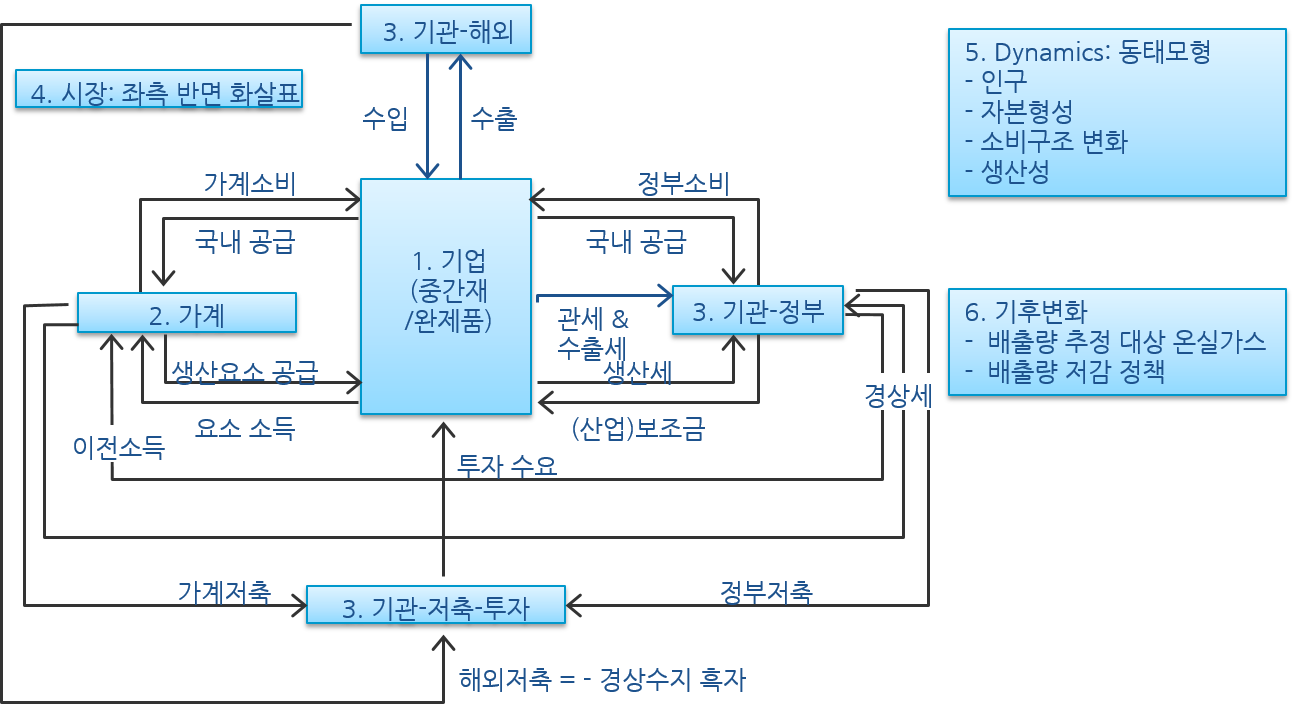
\includegraphics[width=1.00\textwidth]{CGEflow.png}
	\end{figure}
\end{frame}
%----------------------------------------------------------------------------------------------


%------------------------------- 슬라이드  --------------------------------------------------
\begin{frame}
	\frametitle{2010 SAM}
		  	\begin{figure}
	\centering
	 \includegraphics[width=1.00\textwidth]{SAMex.png}
	\end{figure}
\end{frame}
%----------------------------------------------------------------------------------------------

%------------------------------- 슬라이드  --------------------------------------------------
\begin{frame}
	\frametitle{2010 온실가스-산업연관표 }
		  	\begin{figure}
	\centering
	 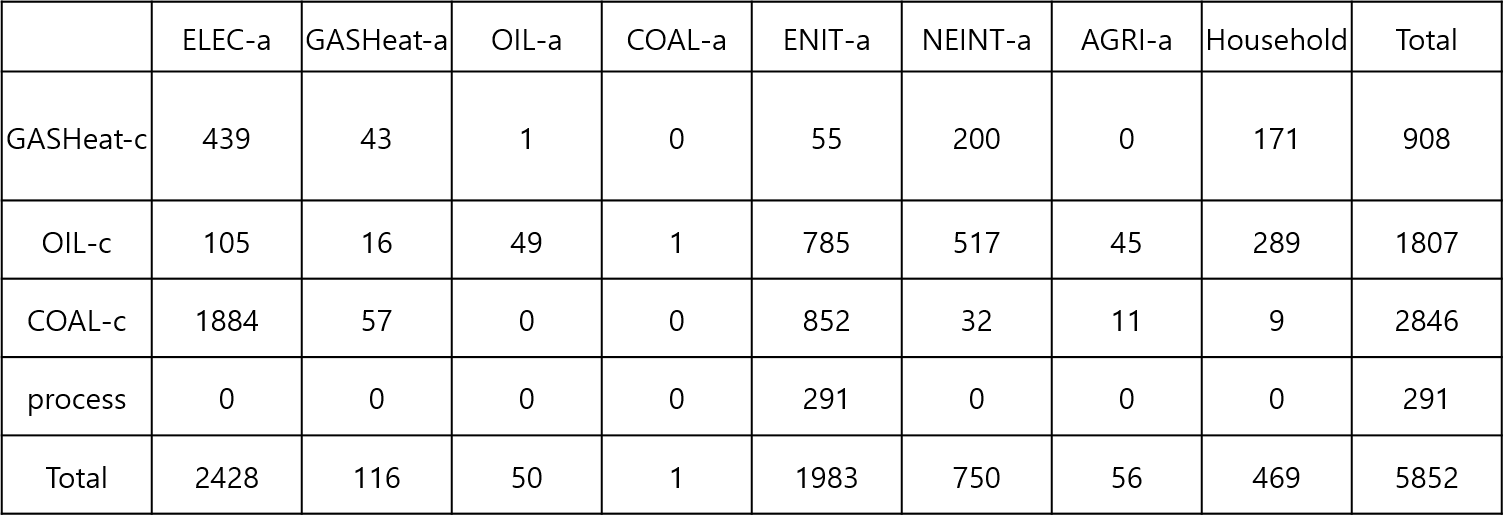
\includegraphics[width=1.00\textwidth]{GHGIO.png}
	\end{figure}
\end{frame}
%----------------------------------------------------------------------------------------------



%------------------------------- 슬라이드  --------------------------------------------------
\begin{frame}
	\frametitle{Toy 생산함수: All ind}
		  	\begin{figure}
	\centering
	 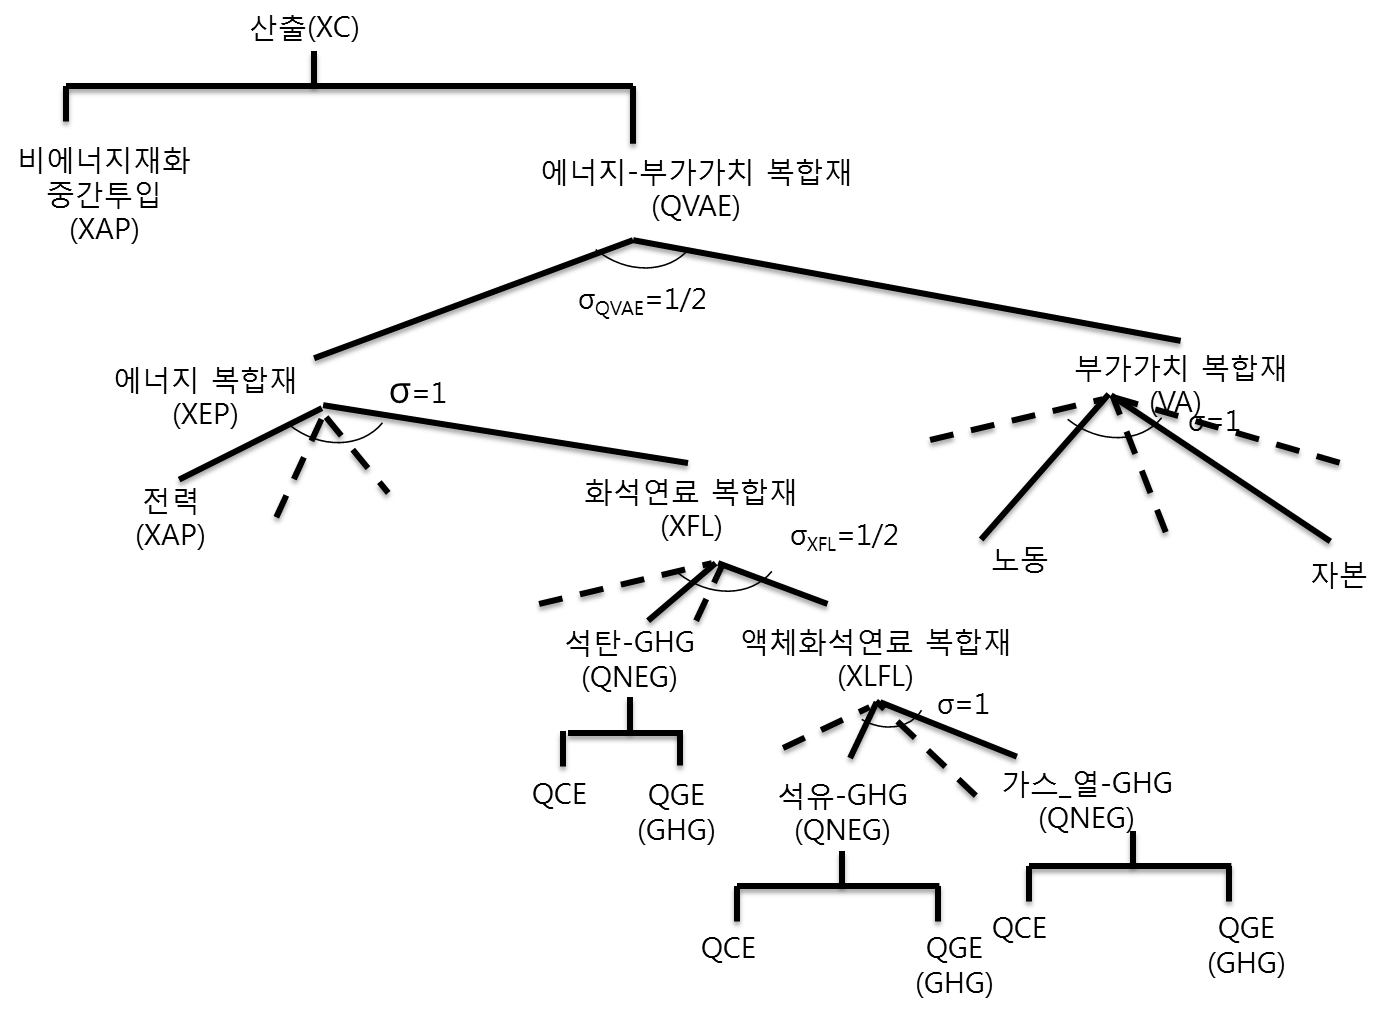
\includegraphics[width=1.00\textwidth]{toypro.png}
	\end{figure}	
\end{frame}
%----------------------------------------------------------------------------------------------

%------------------------------- 슬라이드  --------------------------------------------------
\begin{frame}
	\frametitle{표준모형 생산함수: All ind}
		  	\begin{figure}
	\centering
	 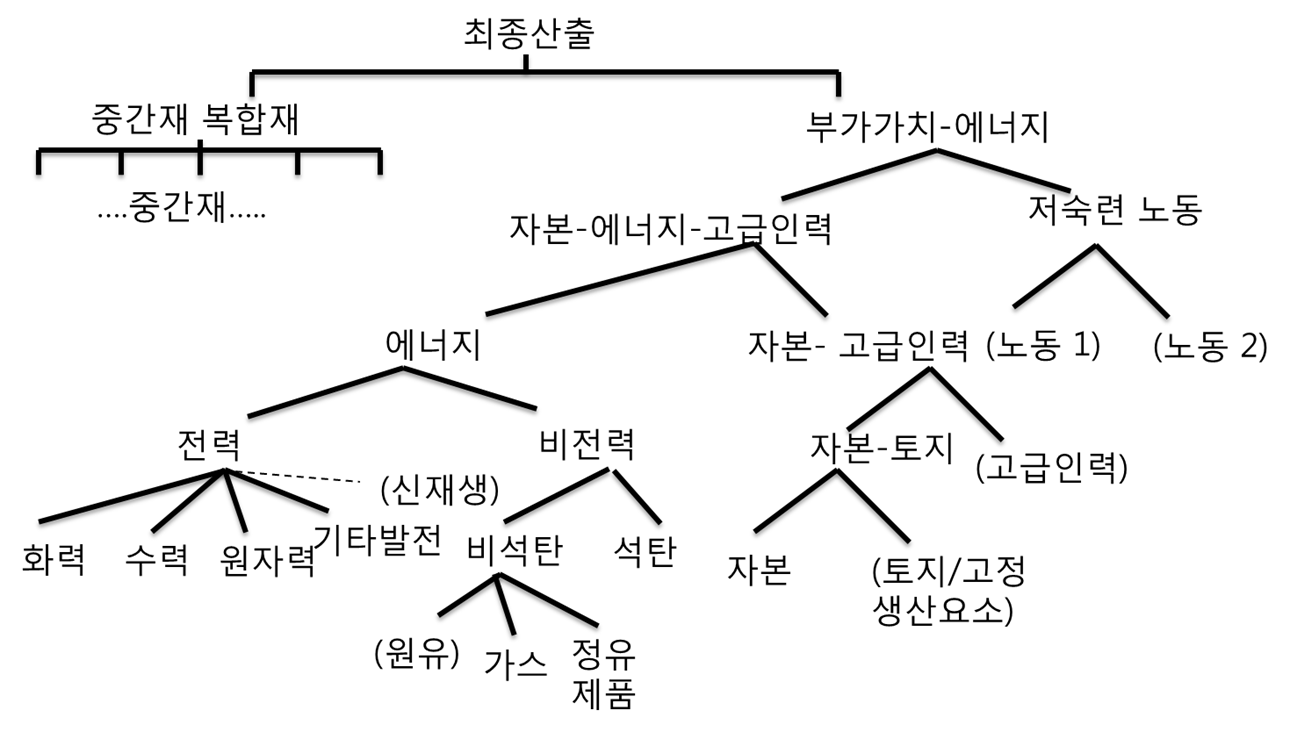
\includegraphics[width=1.00\textwidth]{stpro.png}
	\end{figure}	
\end{frame}
%----------------------------------------------------------------------------------------------

% ******************************
\section{Model Equations and GAMS code}
%*******************************


%*******************************
\subsection{GAMS program 구조}
% ******************************


%------------------------------- 슬라이드  --------------------------------------------------
\begin{frame}[fragile]
\frametitle{GAMS program 구조 (1):Declaration}
\begin{scriptsize}
\begin{enumerate}
\item{Title}
\begin{verbatim}
$TITLE Hybrid model top down module trial version
\end{verbatim}
\item{Declaration: Set}

\begin{verbatim}
SET
A(AC) /ELEC-a,GASHeat-a,OIL-a,COAL-a,ENIT-a,NEINT-a,AGRI-a /
\end{verbatim}
\item{Declaration: Parameter}
\begin{verbatim}
PARAMETERS
alpha_nres(A) net residue to output ratio
\end{verbatim}
\item{Declaration: Variable}
\begin{verbatim}
Variables
VA(A)                  Demand for Value Added composite
\end{verbatim}
\item{Data loading}
\begin{verbatim}
table sam(ACT,ACTP) data in CSV format
$Ondelim
$include b_sam_br_g.csv
$Offdelim
\end{verbatim}

\item{Declaration:Equation}
\begin{verbatim}
Equations
AspPr(C) Absorption Price PA f of PD and PMT;
AspPr(C)$((SAM('ROW',C) ne 0) and (sum(A,SAM(A,C))>0))..
(1/alphaq(C))*(((deltaq(C))**(sigmaq(C))*(PD(C))
\end{verbatim}
\end{enumerate}
\end{scriptsize}
\end{frame}
%------------------------------- 슬라이드  --------------------------------------------------

%------------------------------- 슬라이드  --------------------------------------------------
\begin{frame}[fragile]
\frametitle{GAMS program 구조 (2): Solving Model}
\begin{scriptsize}
\begin{enumerate}
\item{calibration and initialization}
\begin{verbatim}
PC0(A)=1;
\end{verbatim}
\item{Declaration: Model}
\begin{verbatim}
Model
BR 7 ind model
/ImPr.XMT
ResI/;
\end{verbatim}
\item{setting up initial values}
\begin{verbatim}
PC.L(A)        =        PC0(A)        ;
\end{verbatim}
\item{solve and save results}
\begin{verbatim}
Loop (t,SOLVE BR Using MCP;
PCREP(A,t)        =        PC.L(A)        ;
Ks.Fx('Capital')=Ks.L('Capital')*(1-delta)+sum(C,XAF.L('S-I',C));
);
\end{verbatim}
\item{display results}
\begin{verbatim}
display warlasrep;
\end{verbatim}
\item{export output}
\end{enumerate}
\end{scriptsize}
\end{frame}
%------------------------------- 슬라이드  --------------------------------------------------

%*******************************
\subsection{Production}
% ******************************
%------------------------------- 슬라이드  --------------------------------------------------
\begin{frame}
\frametitle{Production: zero profit + input demand}
%\begin{scriptsize}
\bigskip
\begin{enumerate}
\item{각각의 nest 마다 가상의 생산자가 존재: 투입재를 조합해서 복합재를 구성}
\bigskip
\item{Zero profit condition (Each nest): $P=MC, PQ=TC$}
\bigskip
\item{input demand (Each nest): $X_i^d=f(P_i, P_j, P_q, Q)$}
\bigskip
\end{enumerate}
%\end{scriptsize}
\end{frame}
%------------------------------- 슬라이드  --------------------------------------------------


%------------------------------- 슬라이드  --------------------------------------------------
\begin{frame}[fragile]
\frametitle{Production: Top nest (Leontief), zero profit condition}
\begin{scriptsize}

\begin{eqnarray*}
(ActR_a)& &PC_a\cdot\alpha^{nres}_a\cdot XC_a +\sum_c PA_c\cdot ica_{c,a}XC_a+PVAE_aQVAE_a\\
&\ge& PC_a(1-tain_a-taex_a)XC_a +crevI*crevIw_a*CREV_a\\
\end{eqnarray*}
\begin{verbatim}
ActR(A)$(sum(C,SAM(A,C))>0 and not ghg('process',A))..
PC(A)*alpha_nres(A)*XC(A)
+sum(C$M(C),PA(C)*ica(C,A)*XC(A))
+PVAE(A)*QVAE(A)
=g=
PC(A)*(1-ta_in(A)-ta_ex(A))*XC(A)
+crevI*crevIw(A)*CREV(A);
\end{verbatim}


\begin{eqnarray*}
(ActRp_a)& &PC_a\cdot\alpha^nres_a\cdot XC_a +\sum_c PA_c\cdot ica_{c,a}XC_a+\sum_{gc}\theta^P_{gc,a}XC_a\cdot gtax_{gc}+PVAE_aQVAE_a\\
&\ge& PC_a(1-tain_a-taex_a)XC_a +crevI*crevIw_a*CREV_a
\end{eqnarray*}
\begin{verbatim}
ActRp(A)$(ghg('process',A) ne 0)..
PC(A)*alpha_nres(A)*XC(A)
+sum(C$M(C),PA(C)*ica(C,A)*XC(A))
+sum(GC,thetaP(GC,A)*XC(A)*gtax(GC))
+PVAE(A)*QVAE(A)
=g=
PC(A)*(1-ta_in(A)-ta_ex(A))*XC(A)
+crevI*crevIw(A)*CREV(A);
\end{verbatim}
\end{scriptsize}
\end{frame}
%------------------------------- 슬라이드  --------------------------------------------------

%------------------------------- 슬라이드  --------------------------------------------------
\begin{frame}[fragile]
\frametitle{Production: Top nest (Leontief), input demand}
\begin{scriptsize}
\begin{eqnarray*}
(QVAED_a)& & QVAE_a=XC_a\\
\end{eqnarray*}
\begin{verbatim}
QVAED(A)$(sum(C,SAM(A,C))>0)..QVAE(A)=e=XC(A);
\end{verbatim}

\begin{eqnarray*}
(INTDM_{c,a})& & XAP_{c,a}=ica_{c,a}XC_a\\
\end{eqnarray*}
\begin{verbatim}
INTDM(C,A)$(M(C) and SAM(C,A)$M(C)>0)..XAP(C,A)=e=ica(C,A)*XC(A);
\end{verbatim}

\begin{eqnarray*}
(INTDG_{gc,a})& & QINTG_{gc,a}=\theta^P_{gc,a}XC_a\\
\end{eqnarray*}
\begin{verbatim}
INTGD(GC,A)$(ghg('process',A)>0)..QINTG(GC,A)=e=thetaP(GC,A)*XC(A);
\end{verbatim}



\end{scriptsize}
\end{frame}
%------------------------------- 슬라이드  --------------------------------------------------

%------------------------------- 슬라이드  --------------------------------------------------
\begin{frame}[fragile]
\frametitle{Production: 에너지-부가가치 복합재 (QVAE:CES)}
\begin{scriptsize}
\begin{enumerate}
\item{Zero Profit condition: $P=MC$ [$VAEPr_a$]}
\begin{eqnarray*}
PVAE_a&=&(1/\alpha^{VAE}_a)\cdot[\delta_{XEP,a}^{\sigma^{VAE}_a} PEP_a^{(1-\sigma^{VAE}_a)}+\delta_{VA,a}^{\sigma^{VAE}_a} PVA_a^{(1-\sigma^{VAE}_a)}]^{1/(1-\sigma^{VAE}_a)}
\end{eqnarray*}

\begin{verbatim}
VAEPr(A)$(sum(C,SAM(A,C))>0)..PVAE(A)=e=(1/alphaaVAE(A))*
(
deltaXEP(A)**sigmaaVAE(A)*PEP(A)**(1-sigmaaVAE(A))
+ deltaVA(A)**sigmaaVAE(A)*PVA(A)**(1-sigmaaVAE(A))
)**(1/(1-sigmaaVAE(A)));
\end{verbatim}
\item{input demand: $VA_a$ [$XVAD_a$], $XEP_a$ [$XEPD_a$]}
\begin{eqnarray*}
(XVAD_a)& &VA_a=\delta_{VA,a}^{\sigma^{VAE}_a}\left[\frac{PVAE_a}{PVA_a}\right]^{\sigma^{VAE}_a}{\alpha^{VAE}_a}^{({\sigma^{VAE}_a}-1)}QVAE_a
\end{eqnarray*}

\begin{verbatim} 
XVAD(A)$(sum(C,SAM(A,C))>0)..
VA(A)=e=(deltaVA(A)**sigmaaVAE(A))*((PVAE(A)/PVA(A))**sigmaaVAE(A))
*( alphaaVAE(A)**(sigmaaVAE(A)-1))*QVAE(A);
\end{verbatim}
\begin{eqnarray*}
(XEPD_a)& &XEP_a=\delta_{XEP,a}^{\sigma^{VAE}_a}\left[\frac{PVAE_a}{PEP_a}\right]^{\sigma^{VAE}_a}{\alpha^{VAE}_a}^{({\sigma^{VAE}_a}-1)}QVAE_a
\end{eqnarray*}

\begin{verbatim} 
XEPD(A)$(sum(C,SAM(A,C))>0)..
XEP(A)=e=(deltaXEP(A)**sigmaaVAE(A))*((PVAE(A)/PEP(A))**sigmaaVAE(A))
*( alphaaVAE(A)**(sigmaaVAE(A)-1))*QVAE(A);
\end{verbatim}
   
\end{enumerate}
\end{scriptsize}
\end{frame}
%------------------------------- 슬라이드  --------------------------------------------------

%------------------------------- 슬라이드  --------------------------------------------------
\begin{frame}[fragile]
\frametitle{Production: 부가가치 복합재 (VA:Cobb-Douglas)}
\begin{scriptsize}
\begin{enumerate}
\item{Zero Profit condition: $P=MC$ [$VAPr_a$]}
\begin{eqnarray*}
(VAPr_a)\qquad PVA_a&=&\prod_k\left[\frac{R_k}{\lambda_k\lambda_{k,a}\delta^f_{k,a}}\right]^{\delta^f_{k,a}}
\prod_l\left[\frac{W_l}{\lambda^T\lambda_a\delta^f_{l,a}}\right]^{\delta^f_{l,a}}
\end{eqnarray*}

\begin{verbatim}
VAPr(A)$(sum(C,SAM(A,C))>0)..PVA(A)=e=
(
     prod(K,(R(K)/(lambdak*lambdaka(A)*deltaf(K,A)))**(deltaf(K,A)))*
     prod(L,(W(L)/(lambdat*lambda(A)*deltaf(L,A)))**(deltaf(L,A)))
);
\end{verbatim}
\item{input demand: $L^d_a$ [$LDA_{l,a}$], $K^d_a$ [$KDA_{k,a}$]}
\begin{eqnarray*}
(LDA_{l,a})& &L^d_a=\delta^f_{l,a}\left[\frac{PVA_a}{W_l}\right]VA_a
\end{eqnarray*}

\begin{verbatim} 
LDA(L,A)$(sum(C,SAM(A,C))>0)..LD(L,A)=e=deltaf(L,A)*(PVA(A)*VA(A))/W(L);
\end{verbatim}

\begin{eqnarray*}
(KDA_{k,a})& &K^d_a=\delta^f_{k,a}\left[\frac{PVA_a}{R_k}\right]VA_a
\end{eqnarray*}

\begin{verbatim} 
KDA(K,A)$(sum(C,SAM(A,C))>0)..KD(K,A)=e=deltaf(K,A)*(PVA(A)*VA(A))/R(K);
\end{verbatim}
   
\end{enumerate}
\end{scriptsize}
\end{frame}
%------------------------------- 슬라이드  --------------------------------------------------

%------------------------------- 슬라이드  --------------------------------------------------
\begin{frame}[fragile]
\frametitle{Production: 에너지 복합재 (XEP:Cobb-Douglas)}
\begin{scriptsize}
\begin{enumerate}
\item{Zero Profit condition: $P=MC$ [$XEPr_a$]}
\begin{eqnarray*}
(XEPr_a)\qquad PEP_a&=&\prod_{c\in ELECC}\left[\frac{PA_c}{\delta^c_{c,a}}\right]^{\delta^c_{c,a}}
\left[\frac{PFL_a}{1-\sum_{c\in ELECC}\delta^c_{c,a}}\right]^{1-\sum_{c\in ELECC}\delta^c_{c,a}}
\end{eqnarray*}

\begin{verbatim}
XEPr(A)$(sum(C,SAM(A,C))>0)..PEP(A)=e=
  prod(C$ELECC(C),(PA(C)/deltaC(C,A))**(deltaC(C,A)))*
(PFL(A)/(1-sum(C$ELECC(C),deltaC(C,A))))**(1-sum(C$ELECC(C),deltaC(C,A)))
;
\end{verbatim}
\item{input demand: $XFL_a$ [$XFLD_a$], $XAP_{c,a|c\in ELECC}$ [$INTDE_{c,a}$] }
\begin{eqnarray*}
(XFLD_a)& &XFL_a=(1-\sum_{c\in ELECC}\delta^c_{c,a})\left[\frac{PEP_a}{PFL_a}\right]XEP_a
\end{eqnarray*}

\begin{verbatim} 
XFLD(A)$(sum(C,SAM(A,C))>0)..
XFL(A)=e=(1-sum(C$ELECC(C),deltaC(C,A)))*(PEP(A)/PFL(A))*XEP(A);
\end{verbatim}

\begin{eqnarray*}
(INTDE_{c,a})& &XAP_{c,a|c\in ELECC}=\delta^c_{c,a}\left[\frac{PEP_a}{PA_c}\right]XEP_a
\end{eqnarray*}

\begin{verbatim} 
INTDE(C,A)$(ELECC(C) and SAM(C,A)$ELECC(C)>0)..
XAP(C,A)=e= deltaC(C,A)*(PEP(A)/PA(C))*XEP(A);
\end{verbatim}
   
\end{enumerate}
\end{scriptsize}
\end{frame}
%------------------------------- 슬라이드  --------------------------------------------------


%------------------------------- 슬라이드  --------------------------------------------------
\begin{frame}[fragile]
\frametitle{Production: 화석연료 복합재 (XFL:CES),Zero Profit Condition}
\begin{scriptsize}
Zero Profit condition: $P=MC$ [$XFLPr0_a$],[$XFLPr1_a$]

\begin{eqnarray*}
(XFLPr0_a)\qquad PFL_{a|sam(coal-c,a)=0}&=&PLFL_a\\
& &\\
(XFLPr1_a)\qquad PFL_{a|sam(coal-c,a)>0}&=&
\end{eqnarray*}
\begin{displaymath}
\left[\sum_{c\in sfule}{\delta^c_{c,a}}^{\sigma^{XLF}_a}\left[\frac{PNEG_{c,a}}{AEEI_{c,a}}\right]^{(1-\sigma^{XLF}_a)}+(1-\sum_{c\in sfule}\delta^c_{c,a})^{\sigma^{XLF}_a}{PLFL_a}^{(1-\sigma^{XLF}_a)}\right]^{1/(1-\sigma^{XFL}_a)}
\end{displaymath}

\begin{verbatim}
XFLPr0(A)$(sum(C$sfuel(C),SAM(C,A)=0))..PFL(A)=e=PLFL(A);


XFLPr1(A)$(sum(C$sfuel(C),SAM(C,A) >0))..PFL(A)=e=
(
sum(C$SfuelA(A,C),
deltaC(C,A)**sigmaaXFL(A)*(PNEG(C,A)/AEEI(C,A))**(1-sigmaaXFL(A)))
+
(1-sum(C$SfuelA(A,C),deltaC(C,A)))**(sigmaaXFL(A))*PLFL(A)**(1-sigmaaXFL(A))
)**(1/(1-sigmaaXFL(A)));

\end{verbatim}
\end{scriptsize}
\end{frame}
%------------------------------- 슬라이드  --------------------------------------------------

%------------------------------- 슬라이드  --------------------------------------------------
\begin{frame}[fragile]
\frametitle{Production: 화석연료 복합재 (XFL:CES), Input demand}
\begin{scriptsize}
Input Demand: $XLFL_a$ [$XLFLD1_a$,$XLFLD0_a$], $QNEG_{c,a|c\in sfuel}$ [$NEGDS_{c,a}$] 
\begin{eqnarray*}
(NEGDS_{c,a})& &QNEG_{c,a|c\in sfuel}={\delta^C_{c,a}}^{\sigma^{XFL}_a}\left[\frac{PFL_a}{PNEG_{c,a}}\right]^{\sigma^{XFL}_a}AEEI_{c,a}^{(\sigma^{XFL}_a-1)}XFL_a
\end{eqnarray*}

\begin{verbatim}
NEGDS(C,A)$(Sfuel(C) and (sum(CP$sfuel(CP),SAM(CP,A)) >0))..
QNEG(C,A)=e=                
(deltaC(C,A)**sigmaaXFL(A))
*((PFL(A)/PNEG(C,A))**sigmaaXFL(A))
*((AEEI(C,A))**(sigmaaXFL(A)-1))
*XFL(A);
\end{verbatim}

\begin{eqnarray*}
(XLFLD1_{a|\sum_{c\in sfuel}sam(c,a)>0})& &XLFL_a={(1-\sum_{c\in sfuel}\delta^C_{c,a})}^{\sigma^{XFL}_a}\left[\frac{PFL_a}{PLFL_{a}}\right]^{\sigma^{XFL}_a}XFL_a
\end{eqnarray*}

\begin{verbatim}
XLFLD1(A)$(sum(C$sfuel(C),SAM(C,A) >0))
..XLFL(A)=e=
(1-sum(C$sfuel(C),deltaC(C,A)))**sigmaaXFL(A)
*(PFL(A)/PLFL(A))**(sigmaaXFL(A))
*XFL(A);
\end{verbatim}

\begin{eqnarray*}
(XLFLD0_{a|\sum_{c\in sfuel}sam(c,a)=0})& &XLFL_a=XFL_a
\end{eqnarray*}


\begin{verbatim}
XLFLD0(A)$(sum(C$sfuel(C),SAM(C,A)=0))
..XLFL(A)=e=XFL(A);
\end{verbatim}

\end{scriptsize}
\end{frame}
%------------------------------- 슬라이드  --------------------------------------------------

%------------------------------- 슬라이드  --------------------------------------------------
\begin{frame}[fragile]
\frametitle{Production: Gas-Oil 복합재 (XLFL:Cobb-Douglas)}


\begin{scriptsize}
\begin{enumerate}
\item{Zero Profit condition: $P=MC$ [$XLFLPr1_a$]}

\begin{eqnarray*}
(XLFLPr1_a)\qquad PLFL_a=\prod_{c\in Lfuel}\left[\frac{PNEG_{c,a}}{\delta^c_{c,a}\cdot AEEI_{c,a}}\right]^{\delta^C_{c,a}}
\end{eqnarray*}

\begin{verbatim}
XLFLPr1(A)$(Lfuelmix(A) eq 1)..PLFL(A)=e=
prod(C$LfuelA(A,C),(PNEG(C,A)/(deltaC(C,A)*AEEI(C,A)))**deltaC(C,A));
\end{verbatim}
\item{Input Demand: $QNEG_{c,a|c \in Lfuel}$ [$NEGDL1_{c,a}$]}
\begin{eqnarray*}
(NEGDL1_{c,a})\qquad QNEG_{c,a|c \in Lfuel}=\delta^C_{c,a}\frac{PLFL_a}{PNEG_{c,a}}XLFL_a
\end{eqnarray*}

\begin{verbatim}
NEGDL1(C,A)$(Lfuel(C) and Lfuelmix(A) eq 1)
..QNEG(C,A)=e=deltaC(C,A)*(PLFL(A)/PNEG(C,A))*XLFL(A);
\end{verbatim}

\end{enumerate}
\end{scriptsize}
\end{frame}
%------------------------------- 슬라이드  --------------------------------------------------

%------------------------------- 슬라이드  --------------------------------------------------
\begin{frame}[fragile]
\frametitle{Production: 화석연료-온실가스 복합재 (QNEG:Leontief)}


\begin{scriptsize}
\begin{enumerate}
\item{Zero Profit condition: $P=MC$ [$NEGPr_{c,a|c\in fuel}$]}

\begin{eqnarray*}
(NEGPr_{c,a})\qquad PNGE_{c,a}=PA_c +\sum_{gc}\theta^E_{gc,c,a}\cdot gtax_{gc}
\end{eqnarray*}

\begin{verbatim}
NEGPr(C,A)$(ghg(C,A)>0)
..PA(C)+sum(GC,thetaE(GC,C,A)*gtax(GC))=e=PNEG(C,A);
\end{verbatim}

\item{Input Demand: $QCE_{c,a|c \in fuel}$ [$NELQCEDL1_{c,a}$], $QGE_{gc,c,a|c\in fuel}$ [$GD_{gc,c,a|c \in fuel}$]}

\begin{eqnarray*}
(NELQCEDL1_{c,a|c \in fuel})&\qquad& QCE_{c,a}=QNEG_{c,a}\\
(GD_{gc,c,a|c \in fuel})&\qquad& QGE_{gc,c,a}=\theta^E_{gc,c,a}QNEG_{c,a}\\
\end{eqnarray*}

\begin{verbatim}
NELQCED(ENC,A)$(SAM(ENC,A)>0)
..QCE(ENC,A)=e=QNEG(ENC,A);
GD(GC,ENC,A)$(ghg(ENC,A)>0)
..QGE(GC,ENC,A)=e=thetaE(GC,ENC,A)*QNEG(ENC,A);
\end{verbatim}

\end{enumerate}
\end{scriptsize}
\end{frame}
%------------------------------- 슬라이드  --------------------------------------------------

%------------------------------- 슬라이드  --------------------------------------------------
\begin{frame}[fragile]
\frametitle{Production: 산업산출($XC_a$)= 상품생산($XP_{c|c=a}$)}


\begin{scriptsize}
\begin{enumerate}
\item{Zero Profit condition: $P=MC$ [$ComPr_c$]}

\begin{eqnarray*}
(ComPr_{c,a})\qquad \sum_a\theta_{a,c}PC_a=PP_c
\end{eqnarray*}

\begin{verbatim}
ComPr(C)$(sum(A,SAM(A,C))>0)
..sum(A$XPXC(C,A),theta(A,C)*PC(A))=g=PP(C);
\end{verbatim}

\item{Input Demand: $XC_a$ [$ActDC_a$]}

\begin{eqnarray*}
(ActDC_a)\qquad XC_{a}=\sum_c \theta_{a,c}XP_c
\end{eqnarray*}

\begin{verbatim}
ActDC(A)$(sum(C,SAM(A,C))>0)
..XC(A)=g=sum(C$XPXC(C,A),theta(A,C)*XP(C));
\end{verbatim}

\end{enumerate}
\end{scriptsize}
\end{frame}
%------------------------------- 슬라이드  --------------------------------------------------
% ******************************
\subsection{Trade}
% ******************************

%------------------------------- 슬라이드  --------------------------------------------------
\begin{frame}
	\frametitle{Trade: 해외부문(ROW)+수출 결정}
\bigskip
\begin{enumerate}
\item{해외부문}
		\begin{itemize}
		\item{해외: 수입품을 판매하고 그 수익으로 수출품을 구입하고 나머지를 저축}
		\item{수입: 교역조건에 따라 시장수요의 일부분은 수입하여 충당}
		\item{지출: 교역조건에 따라 수출된 국내산출의 일부분을 구입}
		\item{해외 청산: 수입 = 수출+해외저축} 
		\end{itemize}
\bigskip		
\item{Equations}
		\begin{itemize}
		\item{수입가격: 국제가격과 국내가격 관계}
		\item{수입업자 zero profit: Armington 복합재 가격 결정}
		\item{수입, 국산 수요 결정}
		\item{수출가격: 국제가격과 국내가격 관계}
		\item{국내생산자 zero profit : CET 복합재 가격 결정}
		\item{수출, 내수 공급 결정}
		\item{해외부문 balance}
		\end{itemize}
\end{enumerate}
	
\end{frame}
%----------------------------------------------------------------------------------------------
%------------------------------- 슬라이드  --------------------------------------------------
\begin{frame}
	\frametitle{수입-내수-수출 관계: Armingtion and CET}
		  	\begin{figure}
	\centering
	 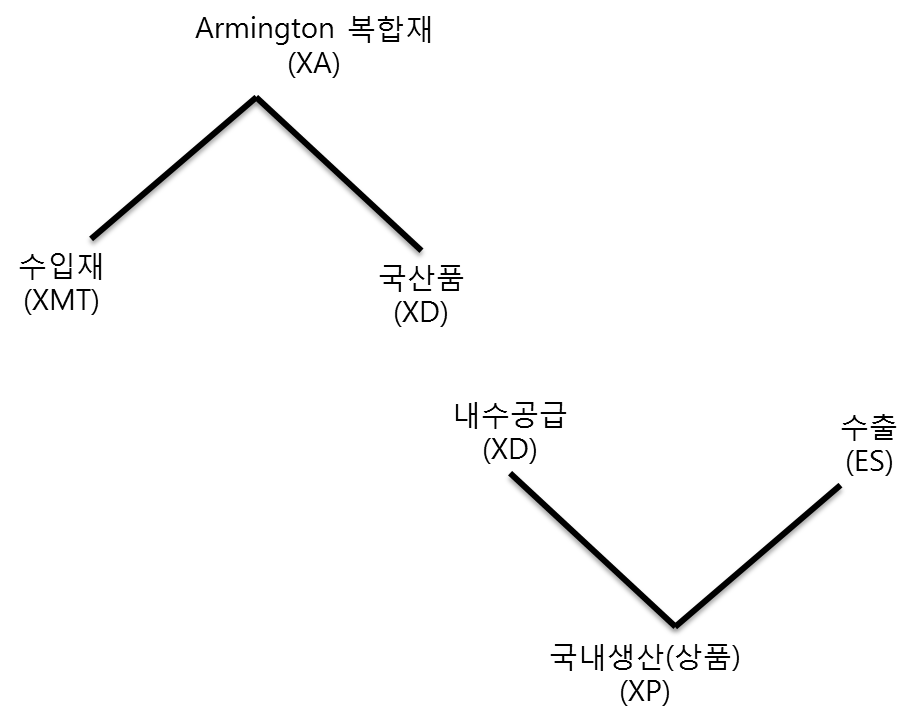
\includegraphics[width=1.00\textwidth]{imex.png}
	\end{figure}	
\end{frame}
%----------------------------------------------------------------------------------------------

%------------------------------- 슬라이드  --------------------------------------------------
\begin{frame}
	\frametitle{수입의 결정: Armington 복합재 생산의 input demand }

\begin{itemize}
	\item{수입가격: 해외가격에 환율을 적용한 국내가를 지불하고 수입세를 납부한 후 소비자가격에 전가}
	\item{총수요-수입수요-내수수요 관계식: 수입업자 zero profit condition}
	\begin{eqnarray*}
 		PA_cXA_c=PD_cXD_c +PMT_cXMT_c\\
	\end{eqnarray*}	
	\item{수입, 내수 수요::주어진 총수요를 충당하는데 비용을 최소화하는 내수-수입 조합 = Armington 복합재 생산}
	\begin{eqnarray*}
 		\min& &PD_cXD_c +PMT_cXMT_c\\
    		& & s.t\quad XA_c=\alpha^{q}_{c}(\delta^{q}_c XD^{-\rho^{q}_c}_c + (1-\delta^{q}_c)XMT^{-\rho^{q}_c}_c)^{-\frac{1}{\rho^{q}_c}}\\
	\end{eqnarray*}
\end{itemize}
\end{frame}
%----------------------------------------------------------------------------------------------



%------------------------------- 슬라이드  --------------------------------------------------
\begin{frame}[fragile]
	\frametitle{수입업자= Armington 복합재 생산자, zero profit condition}
\begin{scriptsize}
\begin{enumerate}
		\item{수입재 국내가격 [$ImPr_c$]}
\begin{displaymath}
(ImPr_c)\qquad pwm_c(1+tm_c)EXR=PMT_c
\end{displaymath}

\begin{verbatim}
ImPr(C)$(SAM('ROW',C) ne 0)..pwm(C)*(1+tm(C))*EXR=g=PMT(C);   
\end{verbatim}
		\item{zero profit condition: $P=MC$ [$AspPr_c$]}

\begin{eqnarray*}
(AspPr_c)& &\\
PA_c&=&(1/\alpha^q_c)[{\delta^q_c}^{\sigma^q_c}{PD_c}^{(1-\sigma^q_c)}+{(1-\delta^q_c)}^{\sigma^q_c}{PMT_c}^{(1-\sigma^q_c)}]^{(1/(1-\sigma^q_c))}
\end{eqnarray*}
\begin{verbatim}
				AspPr(C)$((SAM('ROW',C) ne 0) and (sum(A,SAM(A,C))>0))
				..(1/alphaq(C))*
				(((deltaq(C))**(sigmaq(C))*(PD(C))**(1-sigmaq(c))
				+ (1-deltaq(C))**sigmaq(C)*(PMT(C))**(1-sigmaq(c)))
				**(1/(1-sigmaq(C))))=g=PA(C);
\end{verbatim}
\end{enumerate}
\end{scriptsize}
\end{frame}
%----------------------------------------------------------------------------------------------

%------------------------------- 슬라이드  --------------------------------------------------
\begin{frame}[fragile]
	\frametitle{수입업자= Armington 복합재 생산자, input demand}
\begin{scriptsize}
Input demand: $XD_c$ [$XDD_c$] $XMT_c$ [$XMTD_c$]
\begin{eqnarray*}
(XDD_c)& &XD_c={\delta^q_c}^{\sigma^q_c}\left[\frac{PA_c}{PD_c}\right]^{\sigma^q_c}{\alpha^q_c}^{(\sigma^q_c-1)}XA_c
\end{eqnarray*}


\begin{verbatim}
				XDD(C)$((SAM('ROW',C) ne 0) and (sum(A,SAM(A,C))>0))
				..XD(C)
		=g=
		(deltaq(C)**sigmaq(C))*((PA(C)/(PD(C)))**sigmaq(C))
		*(alphaq(C)**(sigmaq(C)-1))*XA(C);
\end{verbatim}

\begin{eqnarray*}
(XMTD_c)& &XMT_c={\delta^q_c}^{\sigma^q_c}\left[\frac{PA_c}{PMT_c}\right]^{\sigma^q_c}{\alpha^q_c}^{(\sigma^q_c-1)}XA_c
\end{eqnarray*}

\begin{verbatim}
XMTD(C)$((SAM('ROW',C) ne 0) and (sum(A,SAM(A,C))>0))
..XMT(C)
=g=
((1-deltaq(C))**sigmaq(C))*((PA(C)/(PMT(C)))**sigmaq(C))
*(alphaq(C)**(sigmaq(C)-1))*XA(C);
\end{verbatim}

\end{scriptsize}
\end{frame}
%----------------------------------------------------------------------------------------------

%------------------------------- 슬라이드  --------------------------------------------------
\begin{frame}
	\frametitle{수출의 결정: 상품생산자의 output diversification }

\begin{itemize}
	\item{수출가격: 수출세를 지불하고 해외가격으로 판매하여 이를 환전한 수입을 취득}
		\begin{itemize}
		\item{해외가격에 대해서는 가격수용자이기 때문에 수출세만큼 손실 발생 }
		\end{itemize}
	\item{총산출-수출공급-내수공급 관계식: 생산자의 revenue max condition}
	\begin{eqnarray*}
 		PP_cXP_c=PD_cXD_c +PET_cES_c\\
	\end{eqnarray*}	
	\item{수출, 내수 공급:주어진 산출물을 판매하여 수익을 극대화하는 수출-내수 조합. CET 햠수 사용}
		\begin{eqnarray*}
\max& &PET_cES_c+PD_cXD_c\\ 
 & & s.t.\quad XP_c=\alpha^{t}_{c}(\delta^{t}_c ES^{\rho^{t}_c}_c + (1-\delta^{t}_c)XD^{\rho^{t}_c}_c)^{\frac{1}{\rho^{t}_c}}\\
    	\end{eqnarray*}
\end{itemize}
\end{frame}
%----------------------------------------------------------------------------------------------

%------------------------------- 슬라이드  --------------------------------------------------
\begin{frame}[fragile]
	\frametitle{생산자 revenue maximization solution}
\begin{scriptsize}
\begin{enumerate}
		\item{수출재 가격 [$ExPr_c$]}
\begin{displaymath}
(ExPr_c)\qquad pwe_c(1-te_c)EXR=PET_c
\end{displaymath}

\begin{verbatim}
ExPr(C)$(SAM(C,'ROW') ne 0)..PET(C)=g=pwe(C)*(1-te(C))*EXR;
\end{verbatim}
		\item{zero profit condition: $P=MC$ [$ProdPr_c$]}

\begin{eqnarray*}
(ProdPr_c)& &\\
PP_c&=&(1/\alpha^t_c)[{\delta^t_c}^{\sigma^t_c}{PET_c}^{(1-\sigma^t_c)}+{(1-\delta^t_c)}^{\sigma^t_c}{PD_c}^{(1-\sigma^t_c)}]^{(1/(1-\sigma^t_c))}\\
& &\\
& &\left(\rho^t_c=1-(1/\sigma^t_c)\qquad\sigma^t_c=\frac{1}{1-\rho^t_c}\right)\\
\end{eqnarray*}
\begin{verbatim}
ProdPr(C)$((SAM(C,'ROW') ne 0) and (sum(A,SAM(A,C))>0))
..PP(C)=g=
(1/alphat(C))*
(((deltat(C))**(sigmat(C))*(PET(C))**(1-sigmat(c))+ 
(1-deltat(C))**(sigmat(C))*(PD(C))**(1-sigmat(c)))
**(1/(1-sigmat(C))));
\end{verbatim}
\end{enumerate}
\end{scriptsize}
\end{frame}
%----------------------------------------------------------------------------------------------

%------------------------------- 슬라이드  --------------------------------------------------
\begin{frame}[fragile]
	\frametitle{생산자의 Supply decision}
\begin{scriptsize}
Output supply : $XD_c$ [$XDS_c$] $ES_c$ [$ESS_c$]
\begin{eqnarray*}
(XDS_c)& &XD_c={(1-\delta^t_c)}^{\sigma^t_c}\left[\frac{PP_c}{PD_c}\right]^{\sigma^t_c}{\alpha^q_c}^{(\sigma^t_c-1)}XP_c
\end{eqnarray*}


\begin{verbatim}
XDS(C)$(SAM(C,'ROW') ne 0)
..((1-deltat(C))**sigmat(C))*((PP(C)/PD(C))**sigmat(C))
*(alphat(C)**(sigmat(C)-1))*XP(C)=g=XD(C);
\end{verbatim}

\begin{eqnarray*}
(ESS_c)& &ES_c={\delta^t_c}^{\sigma^t_c}\left[\frac{PP_c}{PET_c}\right]^{\sigma^t_c}{\alpha^t_c}^{(\sigma^t_c-1)}XP_c
\end{eqnarray*}

\begin{verbatim}
ESS(C)$(SAM(C,'ROW') ne 0)
..(deltat(C)**sigmat(C))*((PP(C)/PET(C))**sigmat(C))
*(alphat(C)**(sigmat(C)-1))*XP(C)=g=ES(C);
\end{verbatim}

\end{scriptsize}
\end{frame}
%----------------------------------------------------------------------------------------------

%------------------------------- 슬라이드  --------------------------------------------------
\begin{frame}[fragile]
	\frametitle{해외: Trade balance}
\begin{small}
\begin{enumerate}
\item{Trade balance [CAB]}
\begin{eqnarray*}
(CAB)\qquad\sum_c pwm_c XMT_c &=&\sum_c pwe_cES_c+FSAV+tm_{in}(\sum_c PMT_cXMT_c/EXR)\\
\end{eqnarray*}

\begin{verbatim}
CAB..
sum(C$(SAM('ROW',C) ne 0),pwm(C)*XMT(C))
=e=
sum(C$(SAM(C,'ROW') ne 0),pwe(C)*ES(C))
+FSAV
+(tm_{in})*(sum(C$(SAM('ROW',C) ne 0),PMT(C)*XMT(C))/EXR);
\end{verbatim}
\item{Trade balance adjustment [ForS]}
\begin{eqnarray*}
(ForS)\qquad FSAV&=&fasv0*FSAD\\
FASD(t+1)&=&FASD(t)\times(1+TBg(t))\\
\end{eqnarray*}
FSAV, EXR 중 하나는 fix. 나머지는 조정되는데 현재 모형은 FSAV가 수출입 전망에 맞추어 모형 외부에서 삽입되고 EXR가 조정
\begin{verbatim}
ForS..FSAV=e=fsav0*FSAD; 
FSAD=FSAD*(1+TBg(t));
\end{verbatim} 
\end{enumerate}
\end{small}
\end{frame}
%----------------------------------------------------------------------------------------------


% ******************************
\subsection{Household}
% ******************************
%------------------------------- 슬라이드 --------------------------------------------------
\begin{frame}
\frametitle{가계: Income balance + Consumption Demand}
%\begin{scriptsize}
\bigskip
\begin{enumerate}
\item{소득 수취 $\rightarrow$ 감가상각(강제저축) $\rightarrow$ 조세지불$\rightarrow$소비, 재량저축}
\begin{itemize}
\item{소득 = 요소소득 + 이전소득 + 잔폐물 판매소득}
\item{소득세 = 소득세율*(소득-감가상각)}
\item{가처분소득 = (1-소득세율)*(소득-감가상각)}
\item{소비 = 한계소비성향*가처분소득}
\item{저축 = 한계저축성향*가처분소득+감가상각}
\end{itemize}
\bigskip
\item{Equations}
	\begin{itemize}
	\item{재량소비, 재량저축: Roy's identity}
	\item{income balance: Roy's identity를 사용하면 redundant. 포함되지 않음}
	\item{소득, 총저축 정의식은 포함}
	\end{itemize}
\end{enumerate}
%\end{scriptsize}
\end{frame}
%----------------------------------------------------------------------------------------------
%------------------------------- 슬라이드 
\begin{frame}[fragile]
\frametitle{가계:Income definition}
\begin{scriptsize}
\begin{enumerate}
\item{요소소득 : $LY_h$ [$HouseLY_h$], $KY_h$ [$HouseKY_h$]}

\begin{eqnarray*}
(HouseLY_h)&\quad& LY_h=\sum_L shr_{L,h}L^s_lW_l\\
(HouseKY_h)&\quad& KY_h=\sum_K shr_{K,h}K^s_kR_k
\end{eqnarray*}
\begin{verbatim}
HouseLY(H)..LY(H)=e=sum(L,shr(L,H)*Ls(L)*W(L));
HouseKY(H)..KY(H)=e=sum(K,shr(K,H)*Ks(K)*R(K));
\end{verbatim}

\item{이전소득 : $TR_h$ [$Tras_h$]}
\begin{displaymath}
(Tras_h)\quad TR_h=tr0_{per,h}\cdot cpi\cdot Oldpop +crev_h\cdot crevhshr_h\cdot TCREV
\end{displaymath}
\begin{verbatim}
Tras(H)..Tr(H)=e=tr0_per(H)*cpi*Oldpop+crevh*crevh_share(H)*TCREV;
\end{verbatim}

\item{총소득: $YH_h$ [$HouseY_h$]}
\begin{displaymath}
(HouseY_h)\quad YH_h=LY_h+KY_h+TR_h+ResinC;
\end{displaymath}
\begin{verbatim}
HouseY(H)..YH(H)=e=LY(H)+KY(H)+TR(H)+ResinC;
\end{verbatim}


\item{가처분소득: $YD_h$ [$HouseYD_h$]}
\begin{displaymath}
(HouseYD_h)\quad YD_h=(1-TINSR)\cdot\left[LY_h+KY_h+TR_h+ResinC-\delta\sum_k shr_{k,h}K^s_k\right]
\end{displaymath}
\begin{verbatim}  
HouseYD(H)..YD(H)
=e=(1-TINSR)*(LY(H)+KY(H)+TR(H)+ResinC-delta*sum(K,shr(K,H)*Ks(K)));
\end{verbatim}
\end{enumerate}
\end{scriptsize}
\end{frame}
%----------------------------------------------------------------------------------------------
\begin{frame}[fragile]
\frametitle{가계:Consumption and Saving}
\begin{scriptsize}\
\begin{enumerate}
\item{consumption: $XAC_{c,h}$ [$HouseD_{c,h}$]}
\begin{displaymath}
(HouseD_{c,h})\quad XAC_{c,h}=\frac{\mu_{c,h}YD_h}{PA_c(1+tc_{in})}
\end{displaymath}

\begin{verbatim}
HouseD(C,H)$(SAM(C,'Household') ne 0)
..XAC(C,H)=e=mu(C,H)*(YD(H)/(PA(C)*(1+tc_{in})));
\end{verbatim}

\item{savings: 한계저축성향, 저축}
\begin{eqnarray*}
(Saver_h)&\quad& MPS_h=\mu^s_h\\
(Hsave_h)&\quad& SH_h=MPS_h\cdot YD_h+\delta\sum_k shr_{k,h}K^s_h
\end{eqnarray*}
\begin{verbatim}
Saver(H)..MPS(H)=e=mus(H);
Hsave(H)..SH(H)=e=MPS(H)*YD(H)+delta*sum(K,shr(K,H)*Ks(K));
\end{verbatim}
\end{enumerate}
\end{scriptsize}
\end{frame}
%----------------------------------------------------------------------------------------------

% ******************************
\subsection{Government}
% ******************************
%------------------------------- 슬라이드  --------------------------------------------------
\begin{frame}
	\frametitle{정부: 수입, 지출, 예산균형}
\begin{enumerate}
\item{정부: 정부수입을 정부소비 및 정부저축에 사용}
		\begin{itemize}
				\item{정부 수입: 조세}
			\begin{itemize}
			\item{수출입: 관세, 수출세}
			\item{간접세: 순생산물세(PTAXin), 기타생산세(PTAXex)}
			\item{탄소세(TCREV)}
			\item{소득세(YTAX)}
			\end{itemize}
		\item{정부 지출: 정부소비, 이전지출}
		    \begin{itemize}
			\item{정부소비:정부가 생산물을 구입하여 시장수요의 일부 구성}
			\item{이전지출:정부가 가계에 소득을 이전}
			\end{itemize}
		\item{정부 예산균형식: 정부수입 = 정부지출 + 정부저축}
	\end{itemize}
\bigskip
\item{Equations}
	\begin{itemize}
	\item{정부 수입}
	\begin{itemize}
	\item{세율 정의식}
	\end{itemize}
	\item{정부 지출: 소비지출, 이전지출}
	\item{예산 균형식 : 정부 저축}
	\end{itemize}
\end{enumerate}		
\end{frame}
%----------------------------------------------------------------------------------------------

%----------------------------------------------------------------------------------------------
\begin{frame}[fragile]
\frametitle{정부:수입}
\begin{scriptsize}
\begin{enumerate}
\item{정부수입: $YG$ [$GovI$]}
\begin{eqnarray*}
(GovI)& &\\
YG&=&\sum_a(tain_a+taex_a)PC_aXC_a+\sum_c(tm_c)\cdot pwm_c\cdot XMT_c\cdot EXR+\sum_c(te_c)\cdot pwe_c\cdot ES_c\cdot EXR\\
&+&TINSR\cdot\left[\sum_h (YH_h-\delta\sum_k shr_{k,h}K^s_k)\right]\\
&+&\sum_{gc,a}gtax_{gc}QINTG_{gc,a}+\sum_{gc,c,a}gtax_{gc}QGE_{gc,c,a}\\
&+&(tc_{in})\sum_{c,h}PA_cXAC_{c,h}+(tg_{in})\sum_cPA_cXAF_{gov,c}+(tiv_{in})\sum_cPA_cXAF_{s-i,c}+(tm_{in})\sum_cPMT_cXMT_c
\end{eqnarray*}

\begin{verbatim}
GovI..YG=e=
sum(A$(sum(C,SAM(A,C))>0),(ta_in(A)+ta_ex(A))*PC(A)*XC(A))
+sum(C$(SAM('ROW',C) ne 0),tm(C)*pwm(C)*XMT(C)*EXR)
+sum(C$(SAM(C,'ROW') ne 0),te(C)*pwe(C)*ES(C)*EXR)
+(TINSR)*sum(H,(YH(H)-delta*sum(K,shr(K,H)*Ks(K))))
+sum((GC,A)$(ghg('process',A)>0),gtax(GC)*QINTG(GC,A))
+sum((GC,C,A)$(ghg(C,A)>0),gtax(GC)*QGE(GC,C,A))
+tc_{in}*sum((C,H)$(SAM(C,'Household') ne 0),PA(C)*XAC(C,H))
+tg_{in}*sum(C$(SAM(C,'Gov') ne 0),PA(C)*XAF('Gov',C))
+tiv_{in}*sum(C$(SAM(C,'S-I') ne 0),PA(C)*XAF('S-I',C))
+tm_{in}*sum(C$(SAM('ROW',C) ne 0),PMT(C)*XMT(C));
\end{verbatim}


\end{enumerate}
\end{scriptsize}
\end{frame}
%----------------------------------------------------------------------------------------------

%----------------------------------------------------------------------------------------------
\begin{frame}[fragile]
\frametitle{정부:지출, 예산균형}
\begin{scriptsize}
\begin{enumerate}
\item{정부 지출: $XAF_{gov,c}$ [$GovE_c$], $TR_h$ [$Tras_h$]}
\begin{eqnarray*}
XAF_{gov,c}&=&qgr0_c\cdot\frac{\sum_cPA_cXA_c}{PA_c(1+tg_{in})}+\frac{qg0_c}{\sum_c qg0_c}\frac{crevc\cdot TCREV}{PA_c(1+tg_{in})}
\end{eqnarray*}
\begin{verbatim}
GovE(C)$(SAM(C,'Gov') ne 0)
..XAF('Gov',C)=e=qgr0(C)*sum(CP,PA(CP)*XA(CP))*(1/(PA(C)*(1+tg_{in})))
+(qg0(C)/sum(CP,qg0(C)))*crevc*TCREV/(PA(C)*(1+tg_{in}));
\end{verbatim}
\item{예산균형: [$GovB$], 정부저축($SG$) 결정}
\begin{eqnarray*}
SG=YG-\sum_cPA_c(1+tg_{in})XAF_{gov,c}-\sum_hTR_h-crevI*TCREV
\end{eqnarray*}

\begin{verbatim}
GovB..SG=e=
YG-sum(C$(SAM(C,'Gov') ne 0),PA(C)*(1+tg_{in})*XAF('Gov',C))
-sum(H,TR(H))-crevI*TCREV;
\end{verbatim}
예산균형은 정부저축 혹은 소득세율을 조정하여 달성. 현재 소득세율이 fix 되어 정부저축이 조정

\item{소득세율: [$Ytax$] 실효소득세율 $TINSR$ 결정 }
\begin{eqnarray*}
(Ytax)\quad TINSR=\frac{\sum_h(YH_h-\delta\sum_k shr_{k,h}K^s_k)*TINS0-crevtax*TCREV}{\sum_h(YH_h-\delta\sum_k shr_{k,h}K^s_k)}
\end{eqnarray*}
\begin{verbatim}
Ytax..TINSR=e
=(sum(H,(YH(H)-delta*sum(K,shr(K,H)*Ks(K))))*TINS0-crevtax*TCREV)
/sum(H,(YH(H)-delta*sum(K,shr(K,H)*Ks(K))));
\end{verbatim}

\end{enumerate}
\end{scriptsize}
\end{frame}
%----------------------------------------------------------------------------------------------


%------------------------------- 슬라이드  --------------------------------------------------

% ******************************
\subsection{Savings and Investment}
% ******************************

%----------------------------------------------------------------------------------------------
\begin{frame}[fragile]
\frametitle{저축-투자: 투자 결정? Warlas dummy 결정}
\begin{scriptsize}
\begin{enumerate}
\item{저축-투자 부문: 정부, 민간, 해외저축과 투자소비 잔폐물 수입으로 투자재 구입}
\item{투자수요: $XAF_{s-i,c}$ [$Inv_D$] 초기치의 일정 배수}
\begin{eqnarray*}
(InvD_c)& &XAF_{s-i,c}=qinv0_c\cdot IVAD
\end{eqnarray*}
\begin{verbatim}
InvD(C)$(SAM(C,'S-I') ne 0)..XAF('S-I',C)=e=qinv_o(C)*IVAD;
\end{verbatim}
\item{투자-저축 균형: [$InvM$], Warlas dummy ($Warlas$) 결정}
\begin{eqnarray*}
(InvM)& &PA(t+tiv_{in})XAF_{s-i,c}=Warlas+\sum_h SH_h +SG+FSAV*EXR+ResinI;
\end{eqnarray*}
\begin{verbatim}
InvM..
sum(C$(SAM(C,'S-I') ne 0),PA(C)*(1+tiv_{in})*XAF('S-I',C))
=e=Warlas+sum(H,SH(H))+SG+FSAV*EXR+ResinI;
\end{verbatim}
\item{상품시장 청산에 의해 결정된 투자지출의 합은 Warlas=0 인 투자-저축 균형을 만족(Warlas' law)}
\item{개별 투자수요는 상품시장 청산에 의해 결정되는 투자수요의 합을 초기치의 비중에 따라 배분}
\item{현재 저축-투자 청산은 MPS가 고정되어 있어서 IVAD를 조정하여 달성} 
\begin{itemize}
\begin{scriptsize}
\item{투자를 외삽하려면 MPS를 고정시키는 방정식을 없애고 투자를 고정하는 방정식을 도입}
\end{scriptsize}
\end{itemize}
\end{enumerate}
\end{scriptsize}
\end{frame}
%----------------------------------------------------------------------------------------------
% ******************************
\subsection{Market Clearing}
% ******************************

%----------------------------------------------------------------------------------------------
\begin{frame}[fragile]
\frametitle{시장청산조건: 요소시장}
\begin{scriptsize}
\begin{enumerate}
\item{요소시장: 기업의 요소수요의 합 = 요소공급 [$LabM_l$,$CapM_k$}
\begin{eqnarray*}
(LabM_l)& & L^s_l=\sum_a LD_{l,a}\\
(CapM_k)& & K^s_l=\sum_a KD_{k,a}\\
\end{eqnarray*}
\begin{verbatim}
LabM(L)..Ls(L)=g=sum(A$(SAM(L,A)>0),LD(L,A));
CapM(K)..Ks(K)=g=sum(A$(SAM(K,A)>0),KD(K,A));
\end{verbatim}

\item{요소공급: Reduced form 노동 공급 [$Labsup_l$], Capital Evolution}
\begin{eqnarray*}
(Labsup_l)&\quad& L^s_l=LW^0_l(1-TINSR)\left[\frac{W_l}{cpi}\right]^{\epsilon^L_l}\\
& &K^s_{k,0}=K_0\\
& &K^s_{k,t+1}=(1-\delta)K^s_{k,t}+\sum_cXAF_{s-i,c}
\end{eqnarray*}

\begin{verbatim}
Labsup(L)..Ls(L)=e=Lw0(L)*(((1-TINSR)*(W(L)/cpi))**epsilon_L(L));
Ks.Fx(K)        =        Ks0(K)        ;
Ks.Fx('Capital')=Ks.L('Capital')*(1-delta)+sum(C,XAF.L('S-I',C));
\end{verbatim}
\end{enumerate}

\end{scriptsize}
\end{frame}
%----------------------------------------------------------------------------------------------

%----------------------------------------------------------------------------------------------
\begin{frame}[fragile]
\frametitle{시장청산조건: 생산물시장}
\begin{small}
생산물시장: 국내수요 = 아밍턴 재화 공급\\

[$ComMENCN_c$(화석연료이외),$ComMENC_c$(화석연료)]

\begin{eqnarray*}
(ComMENCN_c)& & XA^c=\sum_a XAP_{c,a} +\sum_h XAC_{c,h}+\sum_{fin=\{gov,s-i\}} XAF_{fin,c}\\
(ComMENC_c)& & XA^c=\sum_a QCE_{c,a} +\sum_h XAC_{c,h}+\sum_{fin=\{gov,s-i\}} XAF_{fin,c}
\end{eqnarray*}

\begin{verbatim}
ComMENCN(C)$(ENCN(C))
..XA(C)=g=sum(A$XAPA(C,A),XAP(C,A))
+sum(H$XACH(H,C),XAC(C,H))+sum(FD$FD_C(C,FD),XAF(FD,C));
ComMENC(C)$(ENC(C))
..XA(C)=g=sum(A$XEPA(C,A) ,QCE(C,A ))
+sum(H$XACH(H,C),XAC(C,H))+sum(FD$FD_C(C,FD),XAF(FD,C));
\end{verbatim}
\end{small}
\end{frame}
%----------------------------------------------------------------------------------------------


%----------------------------------------------------------------------------------------------
% ******************************
\subsection{Etc}
% ******************************

%----------------------------------------------------------------------------------------------
\begin{frame}[fragile]
\frametitle{Etc: Normalization, 잔폐물 수입 }
\begin{scriptsize}
\begin{enumerate}
\item{Normalization [Norm]: cpi =1, $cwrt_c$ guarantees initial period cpi=1}
\begin{eqnarray*}
(Norm)& &cpi=\sum_c PA_c*cwrt_c
\end{eqnarray*}
\begin{verbatim}
Norm..cpi=e=sum(C,PA(C)*cwrt(C));
\end{verbatim}

\item{잔폐물 수입 [ResC, ResI]: sum of residue demand = residue supply from household and investment}
\begin{eqnarray*}
(ResC)& &ResinC=\theta^{Res}_c\cdot\sum_a PC_a\alpha^{nres}_a XC_a\\
(ResI)& &ResinI=\theta^{Res}_{iv}\cdot\sum_a PC_a\alpha^{nres}_a XC_a
\end{eqnarray*}

\begin{verbatim}
ResC..ResinC=e=thetaRes_c
*sum(A$(sum(C,SAM(A,C))>0),PC(A)*alpha_nres(A)*XC(A));
ResI..ResinI=e=thetaRes_iv
*sum(A$(sum(C,SAM(A,C))>0),PC(A)*alpha_nres(A)*XC(A));
\end{verbatim}


\end{enumerate}
\end{scriptsize}
\end{frame}
%----------------------------------------------------------------------------------------------

%----------------------------------------------------------------------------------------------
\begin{frame}[fragile]
\frametitle{Etc: 탄소세수 }
\begin{scriptsize}
Carbon tax revenue [$Creve_a$(no process emission), $Crevp_a$ (with process),$TCREV_{sum}$ (total)]

\begin{eqnarray*}
CREVE_a& & CREV_{a|\mbox{no process emission}}=\sum_{gc}gtax_{gc}[\sum_{c,a}QGE_{gc,c,a}]\\
CREVEP_a& &CREV_{a|\mbox{with process emission}}=\sum_{gc}gtax_{gc}[\sum_{c,a}QGE_{gc,c,a}]+\sum_{gc}gtax_{gc}QINTG_{gc,a}\\
TCREVsum& &TCREV=\sum_a CREV_a
\end{eqnarray*}

\begin{verbatim}
CREVE(A)$(ghg('process',A) eq 0)
..CREV(A)=e=sum(GC,gtax(GC)*sum(C$fuelA(A,C),QGE(GC,C,A)));
CREVP(A)$(ghg('process',A) ne 0)
..CREV(A)=e=sum(GC,gtax(GC)*sum(C$fuelA(A,C),QGE(GC,C,A)))
+sum(GC,gtax(GC)*QINTG(GC,A));
TCREVsum..TCREV=e=sum(A,CREV(A));
\end{verbatim}
\end{scriptsize}
\end{frame}
%----------------------------------------------------------------------------------------------

% ******************************
\subsection{Dynamics}
% ******************************


%----------------------------------------------------------------------------------------------
\begin{frame}[fragile]
\frametitle{Dynamics: 자본, 고용, 노령인구, 노동생산성, 무역수지,탄소세}
\begin{scriptsize}
\begin{eqnarray*}
\mbox{자본}& &K^s_{k,t+1}=(1-\delta)K^s_{k,t}+\sum_cXAF_{s-i,c}\\
\mbox{고용}& &LW^0_{t+1}=LW^0_t\cdot(1+g^L_t)\\
\mbox{노령인구}& &OldPop_{t+1}=OldPop_{t}\cdot(1+g^{OP}_t)\\
\mbox{노동생산성}& &\lambda^{T}_{t+1}=\lambda^{T}_t+lpgrow_t\\
\mbox{무역수지}& &FASD_{t+1}=FASD_t\times(1+g^{TB}_t)\\
\mbox{탄소세}& &gtax_{GC,t+1}=gtax_{gc,t}+gtaxPolicy_{gc,t}
\end{eqnarray*}


\begin{verbatim}
Ks.Fx('Capital')=Ks.L('Capital')*(1-delta)+sum(C,XAF.L('S-I',C));
Lw0(L)=Lw0(L)*(1+lgrow(t));
Oldpop=Oldpop*(1+Oldpopg(t));
FSAD=FSAD*(1+TBg(t));
lambdat=lambdat+lpgrow(t);
gtax(GC)=gtax(GC)+gtax_policy(GC,t);
\end{verbatim}

\end{scriptsize}
\end{frame}
%------------------------------- 슬라이드  
\section{분석 예: 탄소세 도입 결과}
\subsection{가정}
%===============================================
%------------------------------------------------------------------------------
\begin{frame}{인구, 경제성장, 탄소세}
	\begin{itemize}
		\item {고용: 통계청 인구전망에 2010년 연령별 취업률 적용}
		\bigskip
		\item {노령인구: 통계청 인구전망}
		\bigskip
		\item {국제수지:중장기 환경전망 및 대응전략(2012) 위탁연구 성과 활용}
		\bigskip
		\item {경제성장: 2010$\sim$20년간 연평균 3.0\% 성장}
		\bigskip
		\item {탄소세: 2016년 1만원/toe 에서 연 1만원/toe씩 5년간 인상}
		\bigskip
		\item {산업구조는 사전에 설정하지 않았고, AEEI는 불변으로 가정}
	\end{itemize}
\end{frame}
%------------------------------------------------------------------------------
%------------------------------------------------------------------------------
\begin{frame}
	\frametitle{탄소세}
	\begin{figure}
		\centering
		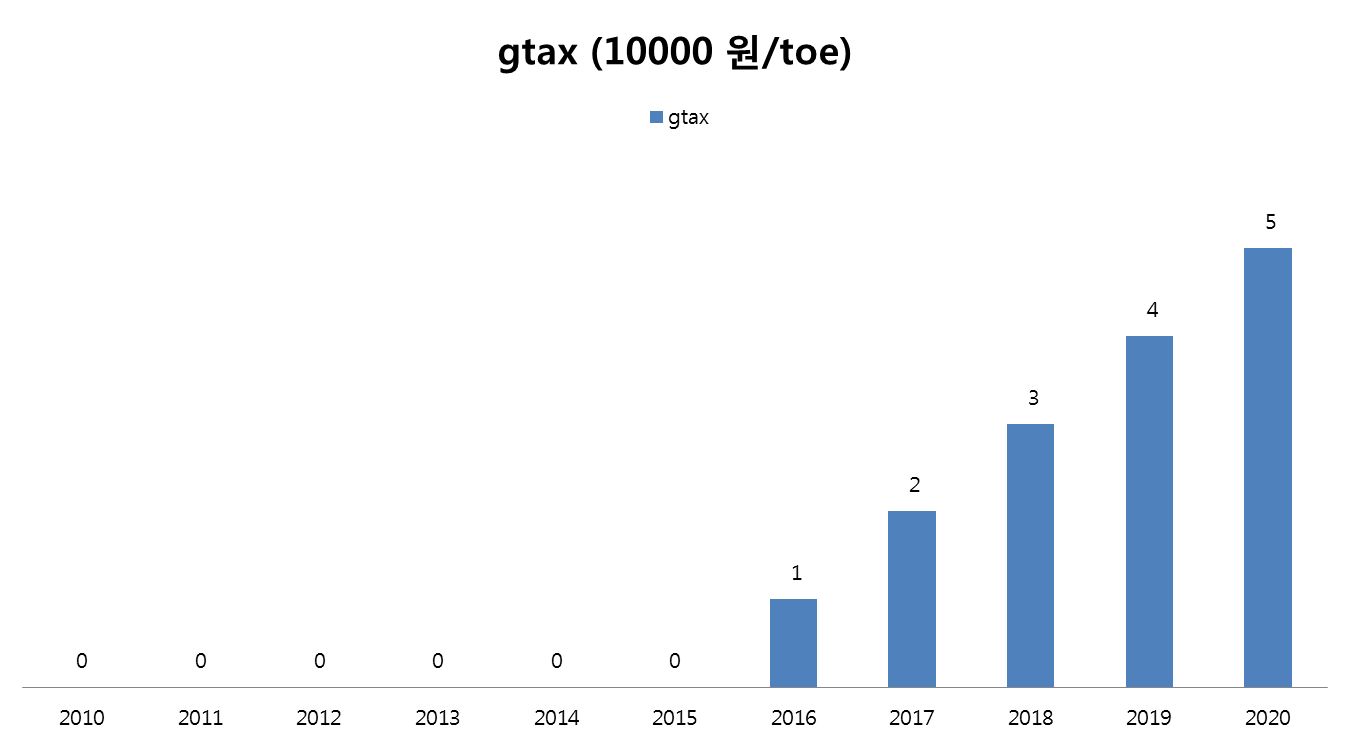
\includegraphics[width=1.00\textwidth]{ctax.png}
	\end{figure}
\end{frame}
%------------------------------------------------------------------------------
%===============================================
	
\subsection{배출량 감축효과}
%------------------------------------------------------------------------------
\begin{frame}
	\frametitle{배출량}
	\begin{itemize}
		\item {2020년 CO2 배출량 19.6\% 감축 가능}
	\end{itemize}
	\begin{figure}
		\centering
		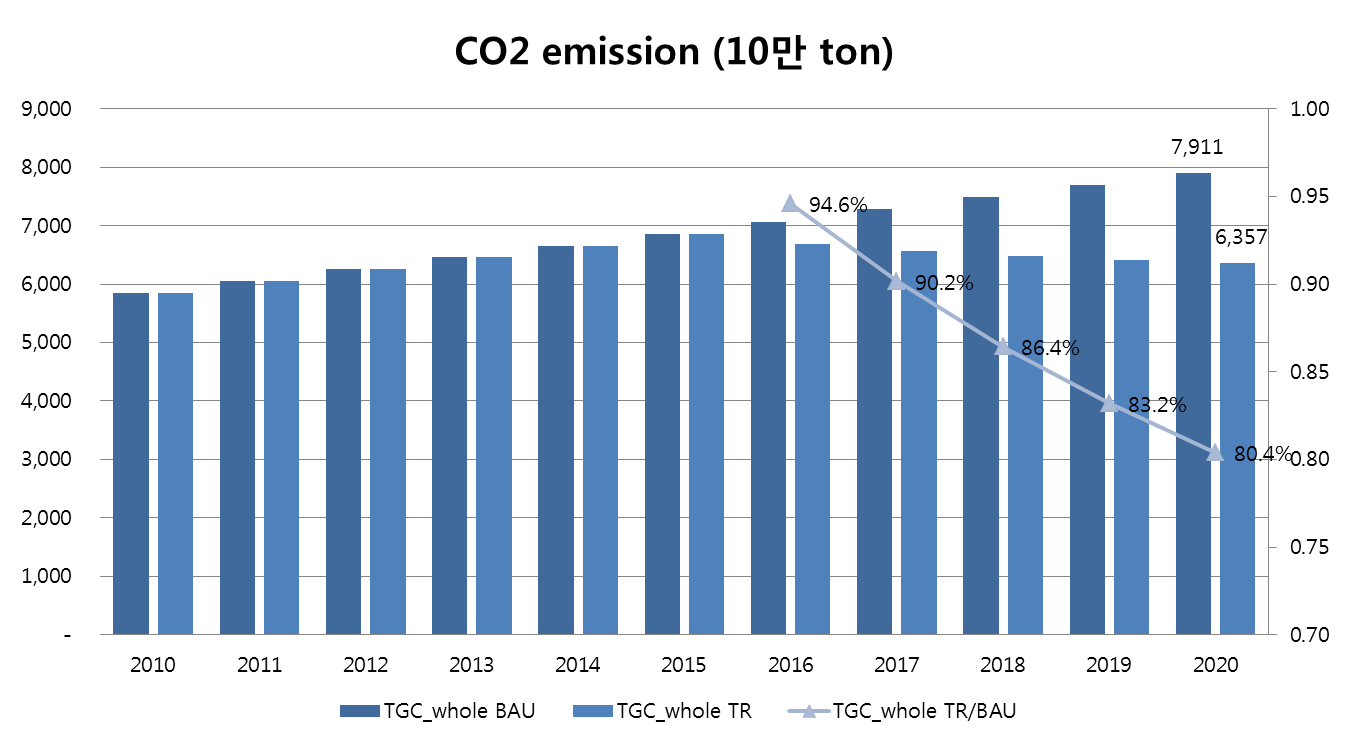
\includegraphics[width=1.00\textwidth]{GHG.png}
	\end{figure}
\end{frame}
%------------------------------------------------------------------------------

%------------------------------------------------------------------------------
\begin{frame}
	\frametitle{원단위배출량}
	\begin{itemize}
		\item {2020년 CO2 배출량/GDP 18.9\% 감축 가능}
	\end{itemize}
	\begin{figure}
		\centering
		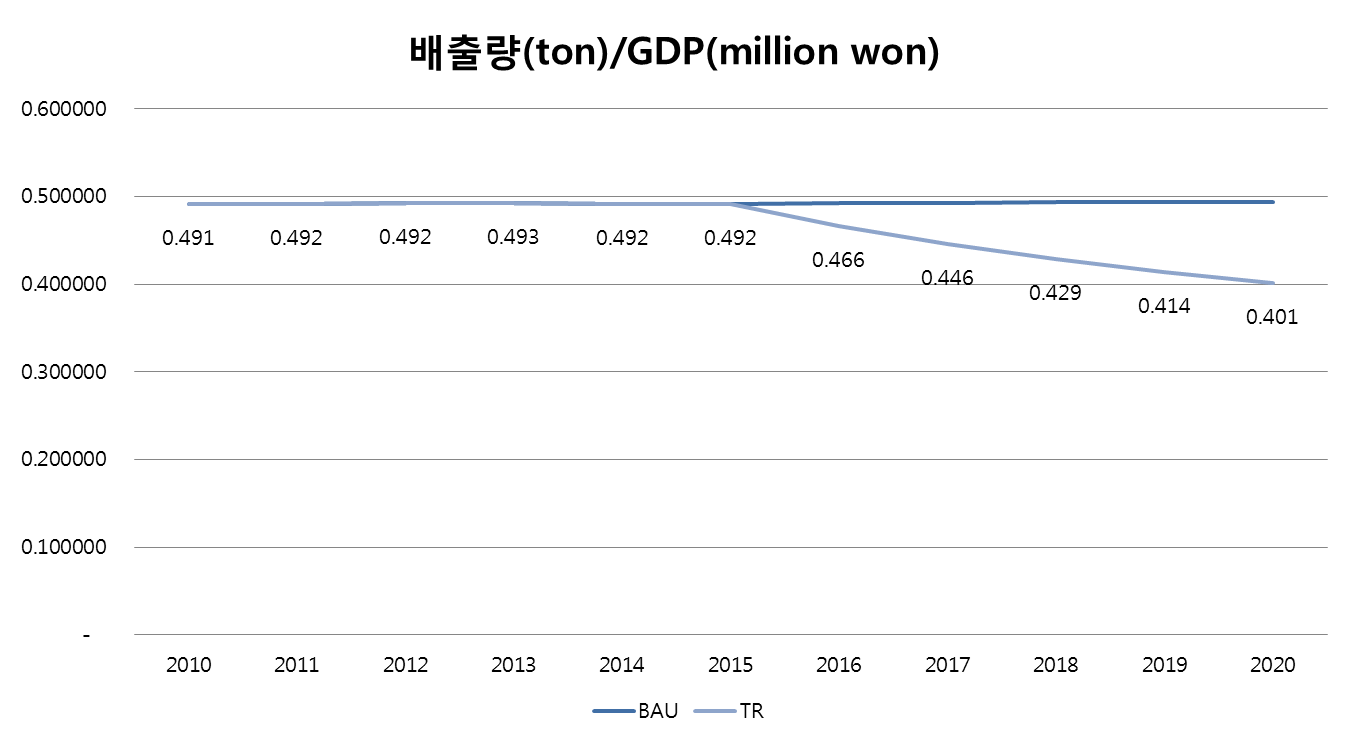
\includegraphics[width=1.00\textwidth]{GHGperOutput.png}
	\end{figure}
\end{frame}
%------------------------------------------------------------------------------

\subsection{정책비용}

%------------------------------------------------------------------------------
\begin{frame}
	\frametitle{GDP loss}
	\begin{itemize}
\item{탄소세로 인한 GDP 손실: BAU GDP 0.18\%(2016)$\sim$0.95\%(2020)}
	\begin{itemize}
		\item {2016$\sim$2020 GDP 손실/BAU GDP 평균= 0.56\%}
		\end{itemize} 	
	\end{itemize}
	\begin{figure}
		\centering
		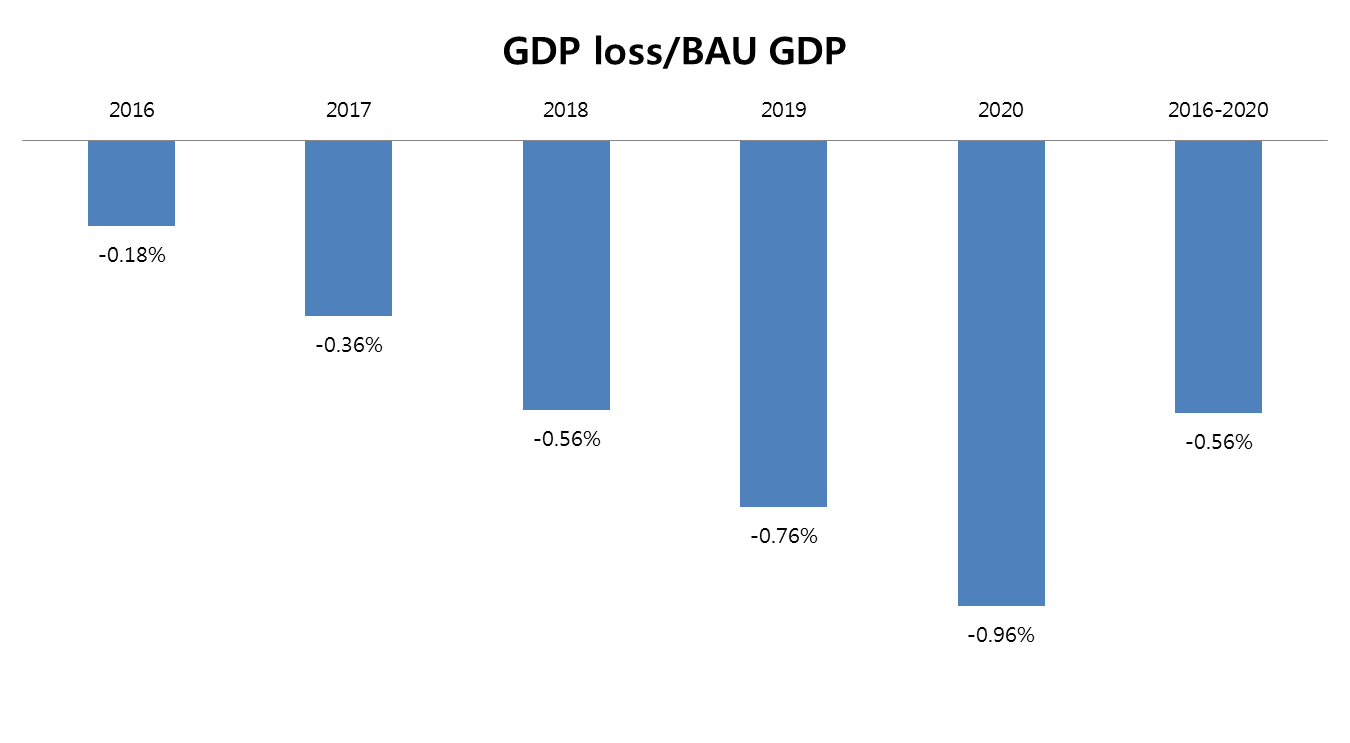
\includegraphics[width=1.00\textwidth]{GDPloss.png}
	\end{figure}
\end{frame}
%------------------------------------------------------------------------------


\subsection{구조변화}
%------------------------------------------------------------------------------
\begin{frame}
	\frametitle{탄소세와 산별 총소비 증가율}
	\begin{itemize}
		\item{에너지 산업 증가율 하락 $>$ 비 에너지 산업 증가율 하락}
		\begin{itemize}
			\item{에너지 산업 share 하락}
		\end{itemize} 
		\bigskip
		\item{비 에너지 Sector: 에너지 집약 산업 증가율 하락$>$ 타 산업 증가율 하락 }
		\begin{itemize}
			\item{에너지 집약 산업 (EINT)share 감소}
		\end{itemize} 	
		\bigskip		
		\item{에너지 Sector: 석탄 증가율 하락 $>$ 기타 에너지 산업 증가율 하락 }
		\begin{itemize}
			\item{석탄 share 감소}
		\end{itemize} 	
	\end{itemize}
\end{frame}
%------------------------------------------------------------------------------

%------------------------------------------------------------------------------
\begin{frame}
	\frametitle{총소비 증가율: 산업}
	\begin{figure}
		\centering
		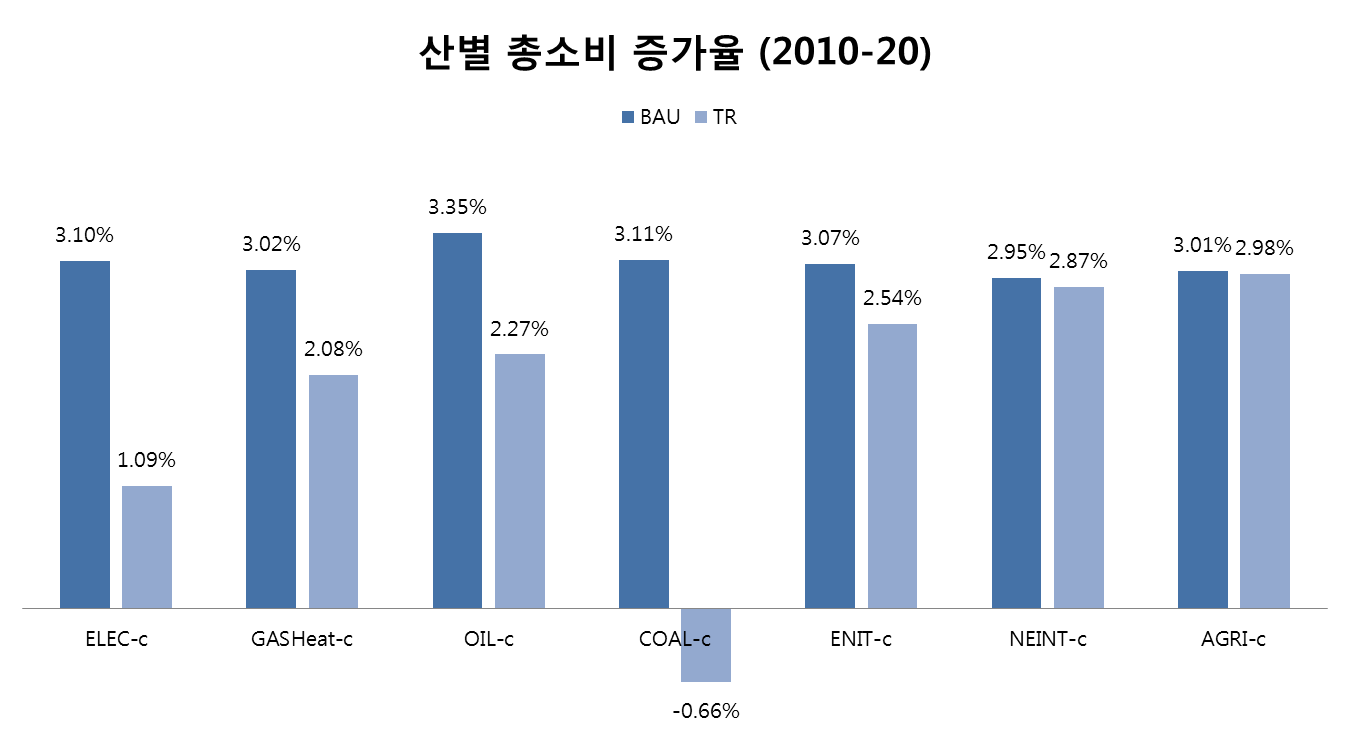
\includegraphics[width=1.00\textwidth]{output_secter.png}
	\end{figure}
\end{frame}
%------------------------------------------------------------------------------

%------------------------------------------------------------------------------
\begin{frame}
	\frametitle{에너지-비에너지 비중 변화}
	\begin{figure}
		\centering
		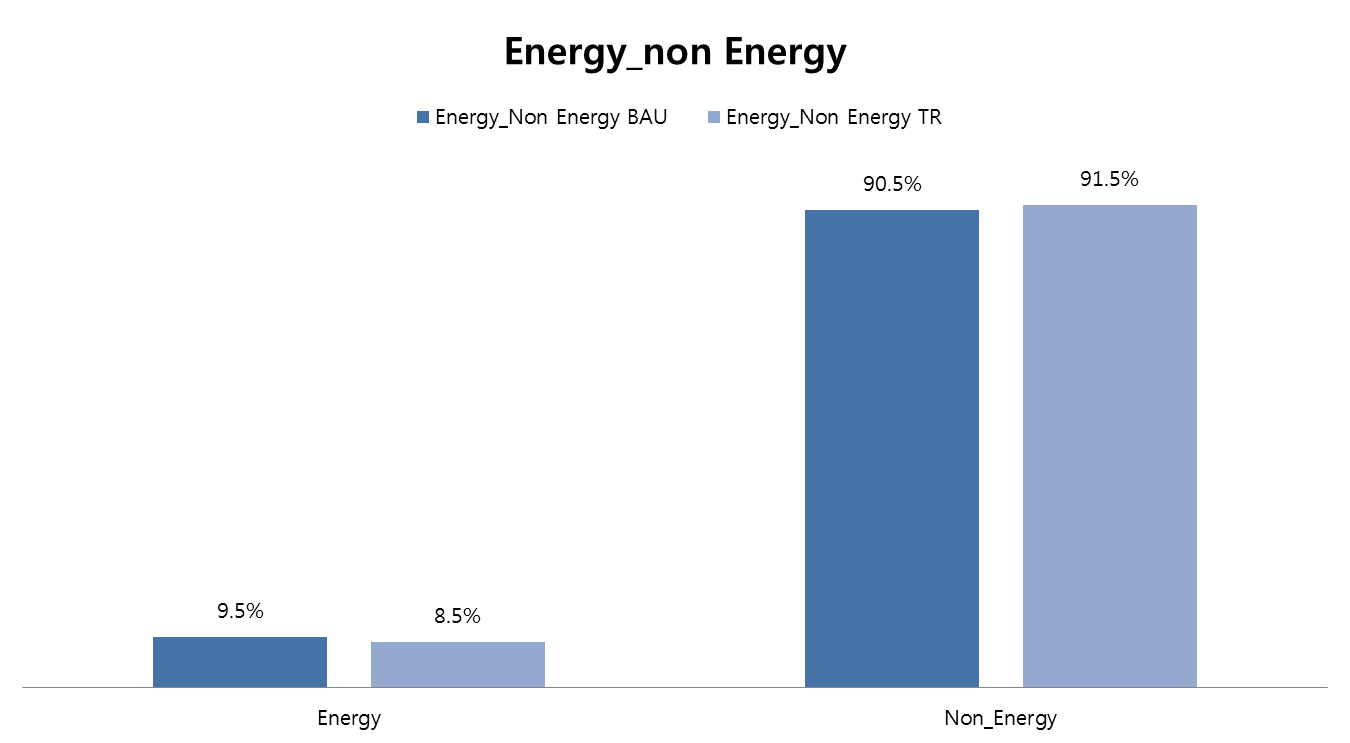
\includegraphics[width=1.00\textwidth]{EandNE.png}
	\end{figure}
\end{frame}
%------------------------------------------------------------------------------

%------------------------------------------------------------------------------
\begin{frame}
	\frametitle{비에너지 secter 비중 변화}
	\begin{figure}
		\centering
		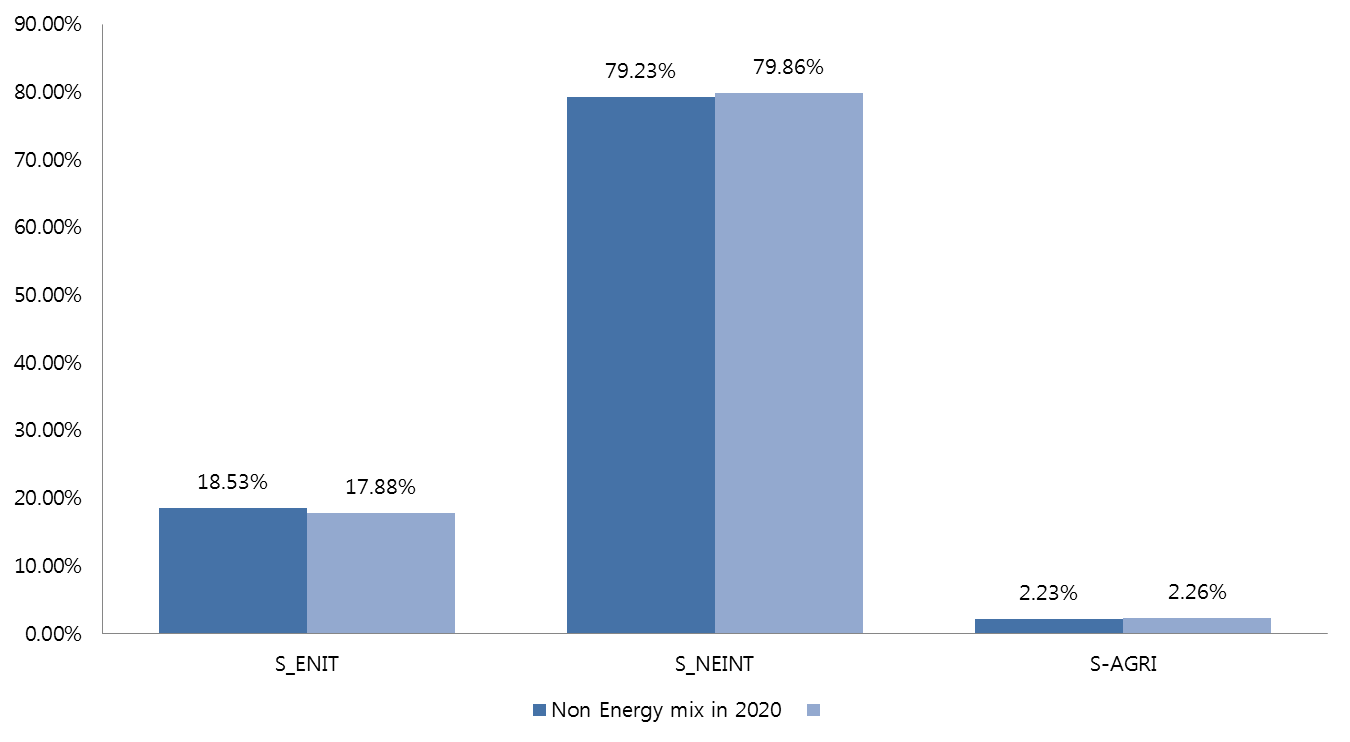
\includegraphics[width=1.00\textwidth]{NEmix.png}
	\end{figure}
\end{frame}
%------------------------------------------------------------------------------

%------------------------------------------------------------------------------
\begin{frame}
	\frametitle{에너지 secter 비중 변화}
	\begin{figure}
		\centering
		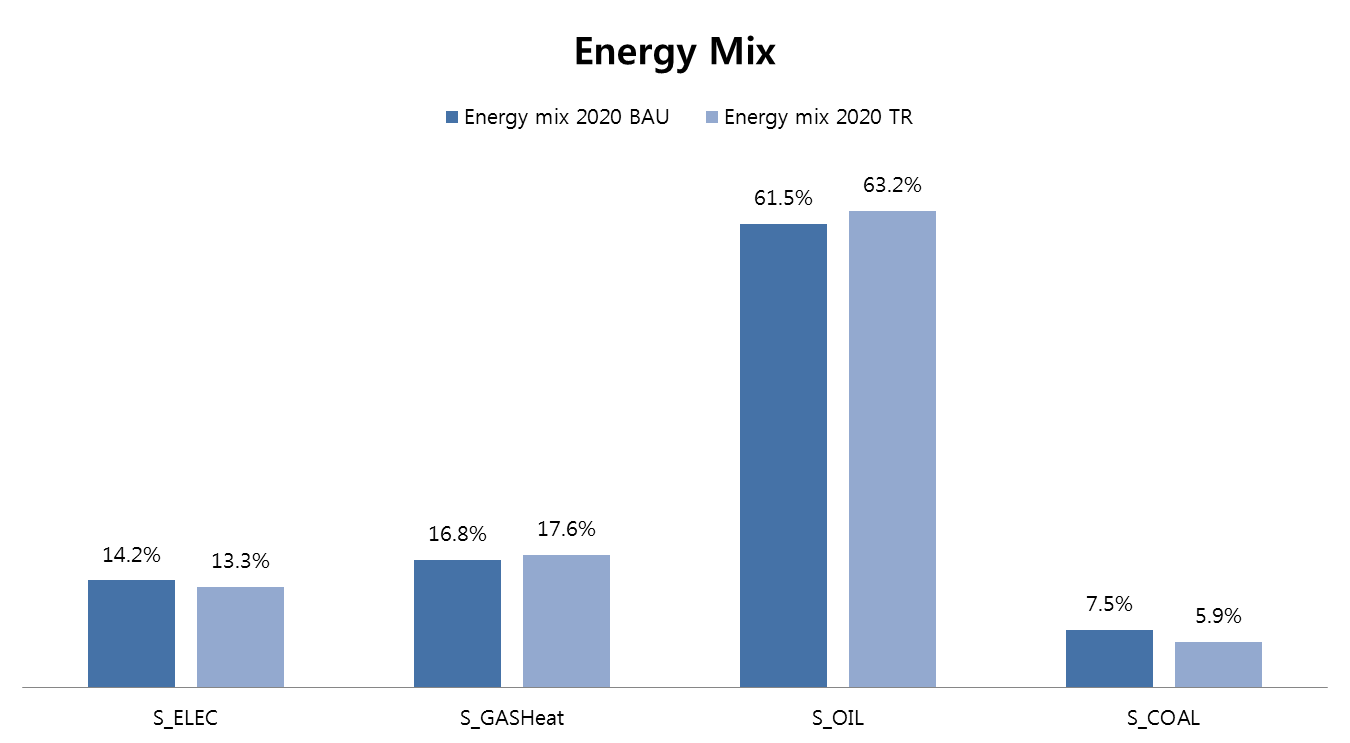
\includegraphics[width=1.00\textwidth]{Emix.png}
	\end{figure}
\end{frame}
%------------------------------------------------------------------------------

%------------------------------------------------------------------------------
\begin{frame}
	\frametitle{Discussion}
		\begin{itemize}
			\item{감축은 Energy mix 변화보다는 산출 하락이 주도}
			\begin{itemize}
				\item{석탄-비석탄 에너지복합재 대체탄력성 0.5: 너무 낮은가?}
			\end{itemize} 
			\bigskip
			\item{에너지 Sector 내에서는 석탄 비중 하락이 뚜렷 }
			\begin{itemize}
				\item{'전력화(Electrification)'현상이 나타나지 않음}
					\begin{itemize}
						\item{전력의 석탄 의존도가 높아서 탄소세부과 이후 타 에너지원 보다 가격경쟁력이 악화}
					\end{itemize} 
				\item{Gas 와 Oil이 비석탄복합재로 석탄과 대체되다 보니 석유의 share가 증가하는 현상 발생}
			\end{itemize} 	
			\end{itemize}
\end{frame}
%------------------------------------------------------------------------------
%------------------------------------------------------------------------------
\begin{frame}
	\frametitle{전력가격/비전력에너지복합재가격}
	\begin{figure}
		\centering
		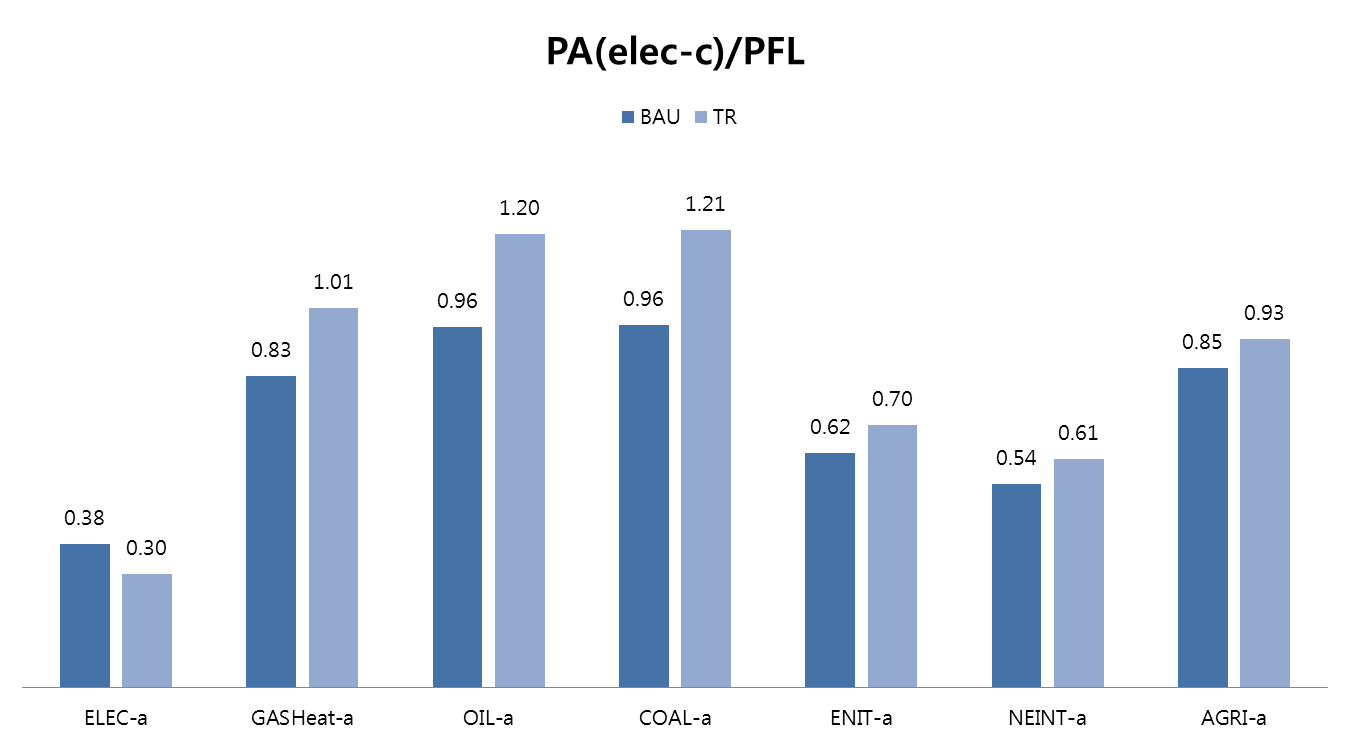
\includegraphics[width=1.00\textwidth]{PelecPFL.png}
	\end{figure}
\end{frame}
%------------------------------------------------------------------------------
%----------------------------------------------------------------------------------------------
\begin{frame}[fragile]
\frametitle{...}
\bigskip
\bigskip
\bigskip
\bigskip
\begin{Huge}
$\qquad$$\qquad$$\qquad$$\qquad$감사합니다.
\end{Huge}
\end{frame}
%----------------------------------------------------------------------------------------------

\end{document}
%==========================  본문 끝 = ================================